\documentclass[12pt,a4paper]{article}
\usepackage[utf8]{inputenc}
\usepackage{amsmath, amssymb, amsfonts}
\usepackage{geometry}
\geometry{margin=2.5cm}
\usepackage{hyperref}
\usepackage{pgfplots}
\usepackage{fancyhdr}
\usepackage{titlesec}
\titleformat{\section}
  {\normalfont\Large\bfseries\centering}  % Format: font size, bold, centered
  {\thesection}{1em}{}
\pagestyle{fancy}
\pgfplotsset{compat=1.18}
\fancyhead{}
\fancyfoot{}
\title{Algebra Lineare}
\author{}
\date{}
\fancyhead[L]{Gabriele Perna}          % Left side
\fancyhead[C]{Algebra lineare}     % Center
\fancyhead[R]{2025/2026}             % Right side
\fancyfoot[C]{\thepage}           % Page number in the center of footer
\let\oldsection\section
\renewcommand{\section}{\clearpage\oldsection}

\begin{document}

\maketitle
\tableofcontents

\section{Sistemi}
\subsection{Sistemi a due variabili}
Se abbiamo un sistema con due equazioni con un totale di 2 variabili, prima si trova il valore di una variabile in funzione dell'altra, si effettua una sostituzione nell'altra equazione e si trovano i valori.

\[
\begin{cases}
x + y = 3 \\
x + 2y = 5
\end{cases}
\]
Effettuiamo il passaggio
\[
\begin{cases}
  x = 3 - y \\
  3 - y + 2y = 5
\end{cases}
\]
Troviamoci i valori
\[
\begin{cases}
  y = 2 \\
  x = 3 - 2 = 1
\end{cases}
\]
Esistono 3 tipi di \textbf{soluzioni} (valori di variabili che soddisfano il sistema) al sistema:
\begin{itemize}
  \item 1 soluzione
  \item Infinite soluzioni
  \item Nessuna soluzione
\end{itemize}
Geometricamente, se consideriamo ogni equazione (che sono rette dato che hanno solo due variabili) come una funzione di cui può essere tracciato il grafico,
ogni soluzione consiste in un punto di \textbf{intersezione} tra le due o più funzioni.

\subsection{Sistemi ed equazioni a tre variabili}
Se un equazione ha 3 variabili, non si parla più di rette su un piano, ma di \textbf{piani nello spazio} tridimensionale
\paragraph{Interpretazione geometrica delle soluzioni:}
\begin{itemize}
  \item \textbf{Retta:} piani intersecati ma non paralleli.
  \item \textbf{0 soluzioni:} piani paralleli ma non intersecati (non lo stesso piano)
  \item \textbf{Un piano:} piani paralleli e intersecati (stesso piano)
\end{itemize}

\subsection{Sistemi a tre equazioni}
Per risolvere sistemi a tre equazioni bisogna prima risolvere le prime due equazioni e poi considerare la terza.
\subsubsection{Sistemi a due variabili}
\paragraph{Le prime due rette intersecate hanno come soluzione una retta}
Si riapplica l'intersezione tra due rette basilare.
\paragraph{Le prime due rette intersecate hanno come soluzione un punto}
\begin{itemize}
  \item \textbf{Un punto:} il punto è contenuto nella terza retta.
  \item \textbf{0 soluzioni:} il punto non è contenuto nella terza retta.
\end{itemize}
\paragraph{Le prime due rette intersecate hanno non hanno soluzione}
Le tre rette intersecate non hanno soluzioni.
\subsubsection{Sistemi a tre variabili}
\paragraph{I primi due piani intersecati hanno come soluzione una retta}
\begin{itemize}
  \item \textbf{Un punto:} la retta interseca in un solo punto nel piano.
  \item \textbf{Retta:} la retta è contenuta nel piano.
  \item \textbf{Nessuna soluzione:} retta parallela al terzo piano
\end{itemize}
\paragraph{I primi due piani intersecati hanno come soluzione un piano}
Si riapplica la basilare intersezione tra due piani.
\paragraph{I primi due piani intersecati non hanno soluzioni}
I tre piani intersecati non hanno soluzioni.

\subsection{Proprietà di sistemi}
\subsubsection{Sistema omogeneo}
Se abbiamo un sistema ad $n$ equazioni lineari con $m$ variabili (caso generale)
\[
\begin{cases}
  a_{11}X_1 + a_{12}X_2 + \cdots + a_{1m}Xm = B1\\
  a_{21}X_1 + a_{22}X_2 + \cdots + a_{2m}Xm = B2\\
  \cdots\\
  a_{n1}X_1 + a_{n2}X_2 + \cdots + a_{nm}Xm = Bn
\end{cases}
\]
Il sistema in questione è \textbf{omogeneo} se:
\[
B_1 = B_2 = \cdots = B_n = 0  
\]
Inoltre, $(0,\ldots,0)$ è sempre soluzione del sistema omogeneo (soluzione \textbf{banale}).
\subsubsection{Sistema omogeneo associato}
Se (E) è un sistema non omogeneo (almeno un $B \ne 0$) allora il suo
sistema omogeneo associato è semplicemente lo stesso sistema ma con tutte le equazioni eguagliate a $0$.
\[
\begin{cases}
  x+y = 3\\
  2x + 3y = 5
\end{cases} 
\]
Sistema omogeneo associato a quello sopra:
\[
\begin{cases}
  x+y = 0\\
  2x + 3y = 0
\end{cases} 
\]
\subsubsection{Soluzioni associate}
Se $(C_1,\ldots,C_m)$ e $(D_1,\ldots,D_m)$ sono soluzioni di un equazione di (E) allora
$(C_1 - D_1,\ldots,C_m - D_m)$ è soluzione della stessa equazione nel sistema omogeneo associato.
\[
\begin{cases}
  a_{11}C_1 + a_{12}C_2 + \cdots + a_{1m}C_m = B1\\
  a_{11}D_1 + a_{12}D_2 + \cdots + a_{1m}D_m = B1\\
  a_{11}(C_1 - D_1) + a_{12}(C_2 - D_2) + \cdots + a_{1m}(C_m - D_m) = B1_{omog} = 0
\end{cases}
\]
Vale ovviamente anche il contrario, ovvero che se $(C_1,\ldots,C_m)$ è soluzione di un equazione di (E) e $(e_1,\ldots,e_m)$ è soluzione
della stessa equazione nel sistema omogeneo associato allora $(C_1 + e_1,\ldots,C_m + e_m)$ è anch'essa soluzione dell'equazione di (E).
\[
\begin{cases}
  a_{11}C_1 + a_{12}C_2 + \cdots + a_{1m}C_m = B1\\
  a_{11}e_1 + a_{12}e_2 + \cdots + a_{1m}e_m = B1_{omog} = 0\\
  a_{11}(C_1 + e_1) + a_{12}(C_2 + e_2) + \cdots + a_{1m}(C_m + e_m) = B1
\end{cases}
\]
\paragraph{Soluzione particolare:} $(C_1,\ldots,C_m)$
\paragraph{Soluzione omogenea:} $(e_1,\ldots,e_m)$
\paragraph{Soluzione generale:} particolare + omogenea\\\\
Esempio: $2x + 3y = 5$
\paragraph{Soluzione particolare:} $(x = 1,y = 1)$
\paragraph{Soluzione omogenea:} $(-\frac{3}{2}y,y)$
\paragraph{Soluzione generale:} $(1,1) + (-\frac{3}{2}y,y) = (1 - \frac{3}{2}y,1 + y)$
\subsubsection{Altre proprietà}
\begin{itemize}
  \item Se scambio due equazioni in un insieme, l'insieme delle soluzioni non cambia.
  \item Se moltiplico una delle equazioni di un insieme per un $k \ne 0$ allora l'insieme delle soluzioni non cambia.
\end{itemize}
\section{Algoritmo di Gauss}
Ogni sistema può essere visto come una matrice di $n$ righe (equazioni) e $m$ colonne (variabili).\\
L'algoritmo di Gauss prende in input una qualsiasi matrice $n * m$ e restituisce una matrice in \textbf{forma a scalini}.\\
Una matrice è in forma a scalini se:
\begin{itemize}
  \item Le righe uguali a $(0,\ldots,0)$ sono in fondo.
  \item Il primo elemento $\ne 0$ di ogni riga (se esiste) è a destra del primo elemento $\ne 0$ della riga precedente, tale elemento si chiama \textbf{pivot}.
\end{itemize}
Esempio di matrice a scalini:
\[
\begin{bmatrix}
1 & 0 & 1 \\
0 & 1 & 0 \\
0 & 0 & 1
\end{bmatrix}
\]
Esempio di matrice NON a scalini (Condizione 2 non soddisfatta):
\[
\begin{bmatrix}
1 & 1 & 1 \\
1 & 1 & 0 \\
0 & 0 & 1
\end{bmatrix}
\]
Le matrici in forma a scalini sono molto facili da risolvere e l'algoritmo di Gauss ci aiuta molto quindi nel risolvere qualsiasi sistema.
\subsection{Applicazione dell'algoritmo a sistemi omogenei}
\begin{enumerate}
  \item Se la matrice è già in forma a scalini, l'algoritmo non si svolge.
  \item Si cerca il primo elemento $\ne 0$ della prima colonna che è $\ne (0,\ldots,0)$.
  \item Si scambia la prima riga con la riga in cui l'elemento è stato trovato, rendendolo il pivot della prima riga.
  \item Si annullano tutti gli elementi sottostanti al pivot (nella stessa colonna) che sono $\ne 0$. Per farlo, si moltiplica la prima riga per un $\lambda ne 0$ e poi si fa la somma con la riga in cui è stato trovato un elemento non nullo nella colonna del pivot, aggiornando tale riga a tale risultato:
  \[
  R_1 \cdot \lambda + R_i
  \]
  Il valore di $\lambda$ è arbitrario, deve riuscire ad annullare gli elementi sotto il pivot.
  \item Si ripete tutto $(2,3,4)$ escludendo la prima riga se la matrice risultante non è ancora in forma a scalini.
\end{enumerate}
Se una volta raggiunta la forma a scalini "perdiamo" qualche variabile (non si presentano
più nelle operazioni) allora vuol dire che possono assumere un qualsiasi valore (soluzioni infinite per quella variabile).\\\\
Se in una matrice in forma a scalini una colonna non ha pivot significa che la variabile caratteristica di quella colonna è detta \textbf{variabile libera} e il risultato dipende dal suo valore. Se c'è almeno una variabile libera in una matrice
in forma a scalini allora esistono infinite soluzioni.
Se invece esiste un pivot per ogni colonna, esiste solo la soluzione banale.
\paragraph{Esempio di esercizio: trasformazione di matrice in forma a scalini:}
\[
\begin{bmatrix}
0 & 0 & 2 & 1 \\
0 & 1 & 4 & 1 \\
0 & 1 & 0 & 1 \\
0 & 2 & 2 & 1
\end{bmatrix}
\]
La matrice non è in forma a scalini, quindi va necessariamente svolto l'algoritmo di Gauss.\\
Eseguendo il passaggio \textbf{N°1}, si trova l'elemento $(R_2,C_2) = 1$.\\
Eseguendo il passaggio \textbf{N°2}, si scambia $R_2$ con $R_1$.
\[
\begin{bmatrix}
0 & 1 & 4 & 1 \\
0 & 0 & 2 & 1 \\
0 & 1 & 0 & 1 \\
0 & 2 & 2 & 1
\end{bmatrix}
\]
Eseguendo il passaggio \textbf{N°3}, si nota che la seconda riga è già pronta, si moltiplica
$R_1$ per $\lambda = -1$ e si effettua la somma con la terza riga, stessa cosa con la quarta riga ma con $\lambda = -2$, eliminando tutti gli elementi sotto il pivot.
\[
\begin{bmatrix}
0 & 1 & 4 & 1 \\
0 & 0 & 2 & 1 \\
0 & 0 & -4 & 0 \\
0 & 0 & -6 & -1
\end{bmatrix}
\]
A questo punto siamo riusciti a compiere un ciclo completo dell'algoritmo, la matrice non è ancora in forma a scalini e bisognerebbe ripetere le operazioni sulla stessa matrice senza la prima riga. (No, non svolgerò un esercizio intero su LaTeX)
\subsection{Applicazione dell'algoritmo a sistemi non omogenei}
Il procedimento per i sistemi non omogenei è lo stesso, però la matrice di partenza vede aggiungersi una colonna, ovvero la colonna dei risultati.
\[
\begin{cases}
  X_1 + X_2 + X_3 + 2X_4 = 9\\
  X_1 + X_2 + 2X_3 + X_4 = 8\\
  X_1 + 2X_2 + X_3 + X_4 = 7\\
  2X_1 + X_2 + X_3 + X_4 = 6
\end{cases}
\]
Diventa:
\[
\begin{bmatrix}
1 & 1 & 1 & 2 \\
1 & 1 & 2 & 1 \\
1 & 1 & 1 & 1 \\
2 & 1 & 1 & 1
\end{bmatrix}
\]
Con l'aggiunta di:
\[
\begin{bmatrix}
9\\
8\\
7\\
6
\end{bmatrix}
\]
Diventando:
\[
\begin{bmatrix}
1 & 1 & 1 & 2 & 9 \\
1 & 1 & 2 & 1 & 8 \\
1 & 1 & 1 & 1 & 7\\
2 & 1 & 1 & 1 & 6
\end{bmatrix}
\]
A questo punto basta applicare il teorema di Gauss per renderla in forma a scalini.
\paragraph{Osservazioni sui risultati:}
\begin{itemize}
  \item \textbf{1 soluzione:} ogni colonna ha un pivot ad esclusione della colonna aggiunta.
  \item \textbf{Infinite soluzioni:} almeno una colonna non aggiunta è senza pivot.
  \item \textbf{0 soluzioni:} la colonna aggiunta ha un pivot.
\end{itemize}
\section{Algoritmo di Gauss-Jordan}
Una matrice è in forma \textbf{ridotta} a scalini se:
\begin{itemize}
  \item Si trova in forma a scalini
  \item Ogni pivot è $= 1$
  \item Ogni pivot è l'unico elemento della propria colonna ad essere $\ne 0$.
\end{itemize}
L'\textbf{algoritmo di Gauss-Jordan} trasforma una matrice in forma ridotta a scalini, ecco il procedimento:
\begin{enumerate}
  \item Si svolge l'algoritmo di Gauss per portare la matrice in forma a scalini, ipotizziamo che questa sia la nostra matrice dopo il primo passo:
  \[
  \begin{bmatrix}
    1 & 2 & 3 & 4\\
    0 & 0 & 2 & 4\\
    0 & 0 & 0 & 3
  \end{bmatrix}
  \]
  \item Moltiplicare le righe dei pivot $\ne 1$ per $\lambda \ne 0$, in questo caso moltiplichiamo la
  seconda riga per $\frac{1}{2}$ e la terza per $\frac{1}{3}$.
  \[
  \begin{bmatrix}
    1 & 2 & 3 & 4\\
    0 & 0 & 1 & 2\\
    0 & 0 & 0 & 1
  \end{bmatrix}
  \]
  \item Si annullano gli elementi $\ne 0$ che sono \textbf{sopra} i pivot, per farlo si moltiplica la riga del pivot e si somma alla riga dell'elemento da annullare, proprio come nell'algoritmo di Gauss, per un $\lambda \ne 0$. Partiamo dal moltiplicare la seconda riga per $\lambda = -3$ e sommiamola alla prima per annullare "3".
  \[
  \begin{bmatrix}
    1 & 2 & 0 & -2\\
    0 & 0 & 1 & 2\\
    0 & 0 & 0 & 1
  \end{bmatrix}
  \]
  Facciamo lo stesso con la terza riga con $\lambda = 2$ per eliminare l'elemento della prima riga e $\lambda = -2$ per eliminare l'elemento della seconda riga. Otteniamo:
  \[
  \begin{bmatrix}
    1 & 2 & 0 & 0\\
    0 & 0 & 1 & 0\\
    0 & 0 & 0 & 1
  \end{bmatrix}
  \]
  Adesso la matrice è in forma ridotta a scalini, una forma estremamente semplice da risolvere.
  \[
  \begin{cases}
    X_1 + 2X_2 = 0\\
    X_3 = 0\\
    X_4 = 0\\
  \end{cases}
  \]
\end{enumerate}
\section{Spazi}
Uno \textbf{spazio k-dimensionale} standard su $\mathbb{R}$ si può definire in questo modo:
\[
\mathbb{R}^n = \{\begin{bmatrix}
    a_1\\
    a_2\\
    a_n
\end{bmatrix}: a_i \in \mathbb{R}\}
\]
Per gli spazi sono valide queste due operazioni:
\begin{enumerate}
  \item \textbf{Somma:}
  \[
  \begin{bmatrix}
    a_1\\
    a_2\\
    ...\\
    a_n
  \end{bmatrix}
   + \begin{bmatrix}
    b_1\\
    b_2\\
    ...\\
    b_n
   \end{bmatrix}
   = \begin{bmatrix}
    a_1 + b_1 \\
    a_2 + b_2 \\
    ...\\
    a_n + b_n
   \end{bmatrix}
  \]
  \item \textbf{Moltiplicazione per} $\lambda \in \mathbb{R}$
  \[
  \begin{bmatrix}
    a_1\\
    a_2\\
    ...\\
    a_n
  \end{bmatrix}
  \cdot \lambda = 
  \begin{bmatrix}
    \lambda a_1\\
    \lambda a_2\\
    ...\\
    \lambda a_n
  \end{bmatrix}
  \]
\end{enumerate}
Per dimostrare queste due operazioni ci aiutiamo con la definizione di \textbf{vettore piano}, ovvero una freccia che parte dall'origine e arriva in un punto.\\
Un vettore è uno spazio bidimensionale $(n = 2)$.
\paragraph{Somma di vettori:}
\[
V_1(a_1, a_2) + V_2(b_1, b_2) = V_3(a_1 + b_1, a_2 + b_2)
\]
\paragraph{Moltiplicazione su vettori:}
\[
V_1(a_1, a_2) \cdot \lambda = V_{1\lambda}(\lambda a_1, \lambda a_2)
\]
Uno \textbf{spazio vettoriale} su $\mathbb{R}$ è un insieme $V$ che ammette le due operazioni in questione, ovvero che:
\begin{itemize}
  \item $V_1,V_2 \in V \implies V_1 + V_2 \in V$
  \item $V_1 \in V, \lambda \in \mathbb{R} \implies V_1 \cdot \lambda \in V$
\end{itemize}
Queste operazioni devono soddisfare i seguenti assiomi:
\begin{itemize}
  \item $(V_1 + V_2) + V_3 = V_1 + (V_2 + V_3)$
  \item $V_1 + V_2 = V_2 + V_1$
  \item $\exists^1 0 \in V : v + 0 = v \forall v \in V$ (esiste solo 1 valore 0)
  \item $\forall v \in V, \exists^1 (-v) : v + (-v) = 0$
  \item $(\lambda_1 + \lambda_2) \cdot v = \lambda_1v + \lambda_2v$
  \item $\lambda(v_1 + v_2) = \lambda v_1 + \lambda v_2$
  \item $(\lambda_1 \cdot \lambda_2) \cdot v = \lambda_1(\lambda_2v)$
  \item $0 \cdot v = 0, (-1)v = -v$
\end{itemize}
Convalidate queste operazioni, $\mathbb{R}^n$ è uno spazio vettoriale su $\mathbb{R}$ dove:
\[
0 = \begin{bmatrix}
  0\\
  0\\
  \ldots\\
  0
\end{bmatrix}
\]
\[
-\begin{bmatrix}
  a_1\\
  a_2\\
  \ldots\\
  a_n
\end{bmatrix}
 = \begin{bmatrix}
  - a_1\\
  - a_2\\
  \ldots\\
  - a_n
 \end{bmatrix}
\]
\subsection{Esempi di somme e moltiplicazioni tra spazi}
\paragraph{Matrici NxM}
\[
A = \begin{bmatrix}
  a_{11} & a_{12} & \ldots & a_{1m} \\
  \ldots\\
  a_{n1} & a_{n2} & \ldots & a_{nm}
\end{bmatrix}
\]
\[
B = \begin{bmatrix}
  a_{11} & a_{12} & \ldots & a_{1m} \\
  \ldots\\
  a_{n1} & a_{n2} & \ldots & a_{nm}
\end{bmatrix}
\]
\[
Somma = \begin{bmatrix}
  a_{11} + b_{11} & a_{12} + b{12} & \ldots & a_{1m} + b_{1m} \\
  \ldots\\
  a_{n1} + b_{n1} & a_{n2} + b_{n2} & \ldots & a_{nm} + b_{nm}
\end{bmatrix}
\]
\[
Moltiplicazione = \begin{bmatrix}
  \lambda a_{11} & \lambda a_{12} & \ldots & \lambda a_{1m} \\
  \ldots\\
  \lambda a_{n1} & \lambda a_{n2} & \ldots & \lambda a_{nm}
\end{bmatrix}
\]
\[
Vettore_0 = \begin{bmatrix}
  0 & 0 & \ldots & 0\\
  \ldots\\
  0 & 0 & \ldots & 0
\end{bmatrix}
\]
\[
-V = \begin{bmatrix}
  -a_{11} & -a_{12} & \ldots & -a_{1m} \\
  \ldots\\
  -a_{n1} & -a_{n2} & \ldots & -a_{nm}
\end{bmatrix}
\]
\paragraph{Polinomi Reali}
\[
A = a_nX^n + a_{n-1}X^{n-1} + \ldots + a_1X + a_0
\]
\[
B = b_mX^m + b_{m-1}X^{m-1} + \ldots + b_1X + b_0
\]
\[
Somma = \begin{cases}
  b_mX^m + \ldots + (b_n + a_n)X^n + \ldots + a_0 + b_0 \impliedby (m > n)\\
  a_nX^n + \ldots + (a_m + b_m)X^n + \ldots + a_0 + b_0 \impliedby (n > m)\\
  (a_n + b_m)X^n + \ldots + a_0 + b_0 \impliedby (m = n)
\end{cases}
\]
\[
Moltiplicazione di A = \lambda a_nX^n + \ldots + \lambda a_0
\]
\[
Vettore_0 = 0
\]
\[
-V = -a_nX^n - a_{n-1}X^{n-1} - \ldots - a_1X - a_0
\]
\subsection{Funzioni continue come spazi vettoriali}
Le funzioni continue formano uno spazio vettoriale su $\mathbb{R}$ con queste operazioni:
\begin{itemize}
  \item $(f_1 + f_2)(x) = f_1(x) + f_2(x)$
  \item $(\lambda f)(x) = \lambda \cdot f(x)$
\end{itemize}
Il vettore 0 di una funzione continua è:
\[
f(x) = 0, \forall x
\]
$-V$ invece è:
\[
(-f)(x) = -f(x)
\]
\section{Sottospazi}
Sia V uno spazio vettoriale. Un \textbf{sottospazio} di V è un sottoinsieme $W \subset V$ tale che:
\begin{itemize}
  \item $V_1,V_2 \in W \implies V_1 + V_2 \in W$
  \item $V_1 \in W, \lambda \in \mathbb{R} \implies \lambda V_1 \in W$.
\end{itemize} 
Un sottoinsieme di uno spazio vettoriale (sottospazio) è sempre uno spazio vettoriale.\\
Se abbiamo un sistema omogeneo, le sue soluzioni formano un sottospazio di $\mathbb{R}^n$\\
Per dimostrare che un insieme è un sottospazio di uno spazio, basta controllare se le operazioni appena enunciate siano veritiere.
\paragraph{Esempio di sottospazio}
\[
\{\begin{bmatrix}
  a_1\\
  a_2\\
  \ldots\\
  a_n
\end{bmatrix}
: a_1 = 0\} \subset \mathbb{R}^n
\]
\[
Somma = \begin{bmatrix}
  0\\
  a_2\\
  \ldots\\
  a_n
\end{bmatrix} + \begin{bmatrix}
  0\\
  b_2\\
  \ldots\\
  b_n
\end{bmatrix} = \begin{bmatrix}
  0\\
  a_2 + b_2\\
  \ldots\\
  a_n + b_n
\end{bmatrix} \in W
\]
\[
Moltiplicazione = \begin{bmatrix}
  0\\
  a_2\\
  \ldots\\
  a_n
\end{bmatrix} \cdot \lambda = \begin{bmatrix}
  0\\
  \lambda a_2\\
  \ldots\\
  \lambda a_n
\end{bmatrix} \in W
\]
\paragraph{Esempio di non sottospazio}
\[
\{\begin{bmatrix}
  a_1\\
  a_2\\
  \ldots\\
  a_n
\end{bmatrix}
: a_1 = 1\} \subset \mathbb{R}^n
\]
\[
Somma = \begin{bmatrix}
  1\\
  a_2\\
  \ldots\\
  a_n
\end{bmatrix} + \begin{bmatrix}
  1\\
  b_2\\
  \ldots\\
  b_n
\end{bmatrix} = \begin{bmatrix}
  2\\
  a_2 + b_2\\
  \ldots\\
  a_n + b_n
\end{bmatrix} \notin W
\]
I sottospazi sono praticamente sottoinsiemi e quindi possiamo applicare le solite operazioni dei sottoinsiemi su di essi.\\
\[
W_1,W_2 \subset V
\]
\[
(W_1 \cap W_2) \subset V 
\]
L'intersezione è un sottospazio, ma l'unione $W_1 \cup W_2$ non è quasi mai un sottospazio.\\
Per esempio se abbiamo $W_1 = y$ e $W_2 = x$, la loro unione non è un sottospazio perchè se sommiamo per esempio:
\[
P_1(0,1) + P_2(1,0) = (1,1) \notin V
\]
\section{Combinazioni lineari}
Nell'esempio precedente, ogni punto di $\mathbb{R}^2$ è contenuto in $W_1 + W_2$ perchè se consideriamo $(a,b)$ come un punto generale in $\mathbb{R}^2$:
\[
(a,b) = a(1,0) + b(0,1) \in W_1 + W_2
\]
Dato $V$ uno spazio vettoriale e $v_1,v_2 \in V$, una \textbf{combinazione lineare} di $v_1 e v_2$ è un vettore della forma:
\[
\lambda_1 \cdot v_1 + \lambda_2 \cdot v_2,
\]
Dove $\lambda_1, \lambda_2 \in \mathbb{R}$\\
Possiamo sostituire infatti $a$ e $b$ con $\lambda_1$ e $\lambda_2$:
\[
(\lambda_1,\lambda_2) = \lambda_1(1,0) + \lambda_2(0,1)
\]
Infatti, ogni punto / vettore del piano è combinazione lineare di $(1,0)$ e $(0,1)$.\\\\
Più in generale, se $v_1,\ldots,v_m \in V$, una combinazione lineare di questi vettori è:
\[
\lambda_1 \cdot v_1 + \cdots + \lambda_m v_m
\]
\[
\forall \lambda \in \mathbb{R}
\]
Il sottospazio di $V$ generato da $v_1,\ldots,v_m \in V$ è:
\[
Span(v_1,\ldots,v_m) = \{\lambda_1 \cdot v_1 + \cdots + \lambda_m \cdot v_m : \lambda_1,\ldots,\lambda_m \in \mathbb{R}\}
\]
Ovvero tutte le combinazioni lineari possibili su tali vettori.
\textbf{Esempio:}
\[
V = \mathbb{R}^2, v_1 = \begin{bmatrix}
  1\\
  0
\end{bmatrix}, v_2 = \begin{bmatrix}
  0\\
  1
\end{bmatrix}
\]
\[
Span(v_1,v_2) = \{\lambda_1 \cdot \begin{bmatrix}
  1\\
  0
\end{bmatrix} + \lambda_2 \cdot \begin{bmatrix}
  0\\
  1
\end{bmatrix}\}
\]
\[
Span(v_1,v_2) = \{\begin{bmatrix}
  \lambda_1\\
  0
\end{bmatrix} + \begin{bmatrix}
  0\\
  \lambda_2
\end{bmatrix}\}
\]
\[
Span(v_1,v_2) = \{\begin{bmatrix}
  \lambda_1\\
  \lambda_2
\end{bmatrix}\}
\]
\paragraph{Esempio:}
\[
V = \mathbb{R}^2, v_1 = \begin{bmatrix}
  0\\
  1\\
  0
\end{bmatrix}, v_2 = \begin{bmatrix}
  0\\
  0\\
  1
\end{bmatrix}
\]
\[
Span(v_1,v_2) = \{\lambda_1 \cdot \begin{bmatrix}
  0\\
  1\\
  0
\end{bmatrix} + \lambda_2 \cdot \begin{bmatrix}
  0\\
  0\\
  1
\end{bmatrix}\}
\]
\[
Span(v_1,v_2) = \{\begin{bmatrix}
  0\\
  \lambda_1\\
  0
\end{bmatrix} + \begin{bmatrix}
  0\\
  0\\
  \lambda_2
\end{bmatrix}\}
\]
\[
Span(v_1,v_2) = \{\begin{bmatrix}
  0\\
  \lambda_1\\
  \lambda_2
\end{bmatrix}\}
\]
\paragraph{Esempio:}
\[
V = \mathbb{R}^2, v_1 = \begin{bmatrix}
  0\\
  1\\
  1
\end{bmatrix}, v_2 = \begin{bmatrix}
  0\\
  0\\
  -1
\end{bmatrix}
\]
\[
Span(v_1,v_2) = \{\lambda_1 \cdot \begin{bmatrix}
  0\\
  1\\
  1
\end{bmatrix} + \lambda_2 \cdot \begin{bmatrix}
  0\\
  0\\
  -1
\end{bmatrix}\}
\]
\[
Span(v_1,v_2) = \{\begin{bmatrix}
  0\\
  \lambda_1\\
  \lambda_1
\end{bmatrix} + \begin{bmatrix}
  0\\
  0\\
  -\lambda_2
\end{bmatrix}\}
\]
\[
Span(v_1,v_2) = \{\begin{bmatrix}
  0
  \lambda_1\\
  \lambda_1 - \lambda_2
\end{bmatrix}\}
\]
Questo si può riscrivere come:
\[
Span(v_1,v_2) = \{\begin{bmatrix}
  0
  a\\
  b
\end{bmatrix}\}
\]
\[
a = \lambda_1, b = \lambda_1 - \lambda_2
\]
Si può concludere che un sottospazio può essere lo span di più di un sistema di vettori.
\section{Dipendenza lineare}
Dato $V$ come spazio vettoriale, $v_1,\ldots,v_m \in V$ sono \textbf{linearmente dipendenti} se esistono $\lambda_1,\ldots,\lambda_m \in \mathbb{R}$ non tutti uguali a $0$ tale che:
\[
\lambda_1 \cdot v_1 + \cdots + \lambda_m \cdot v_m = 0
\]
Altrimenti sono \textbf{linearmente indipendenti}.\\\\
$v_1,\ldots,v_m \in V$ sono linearmente dipendenti se almeno uno tra di loro è combinazione lineare degli altri, vediamo un esempio:
\[
v_1 = \begin{bmatrix}
  0\\
  1\\
  0
\end{bmatrix}, v_2 = \begin{bmatrix}
  0\\
  0\\
  1
\end{bmatrix}, v_3 = \begin{bmatrix}
  0\\
  1\\
  1
\end{bmatrix}
\]
\paragraph{Dimostrazione:}
Se $v_1,\ldots,v_m \in V$ sono linearmente dipendenti, esistono $\lambda_1,\ldots,\lambda_m$ tale che $\lambda_1 \cdot v_1 + \cdots + \lambda_m \cdot v_m = 0$ e per esempio $\lambda_1 = 0$ allora posso dividere tutto per $\lambda_1$:
\[
\lambda_1 \cdot v_1 + \cdots + \lambda_m \cdot v_m = 0
\]
Diventa:
\[
v_1 + \cdots + \frac{\lambda_m}{\lambda_1} \cdot v_m = 0
\]
Si nota che $v_1$ è combinazione lineare degli altri vettori:
\[
v_1 = -\frac{\lambda_2}{\lambda_1} \cdot v_2 - \cdots - \frac{\lambda_m}{\lambda_1} \cdot v_m
\]
Con questo si può concludere che se $\lambda_i \ne 0$ allora $v_i$ è combinazione lineare degli altri.
\subsection{Interpretazione algebrica}
La dipendenza lineare in $\mathbb{R}^n$ si vede in questo modo, prendiamo un esempio:
\[
v_1, \ldots, v_m \in \mathbb{R}^n
\]
\[
v_1 = \begin{bmatrix}
  a_{11}\\
  \ldots\\
  a_{n1}
\end{bmatrix}, \ldots, v_m = \begin{bmatrix}
  a_{1,m}\\
  \ldots\\
  a_{n,m}
\end{bmatrix}
\]
\[
\lambda_1 \cdot v_1 + \cdots + \lambda_m \cdot v_m = 0 \Leftrightarrow \lambda_1 \cdot \begin{bmatrix}
  a_{11}\\
  \ldots\\
  a_{n1}
\end{bmatrix} + \cdots + \lambda_m \cdot \begin{bmatrix}
  a_{1,m}\\
  \ldots\\
  a_{n,m}
\end{bmatrix} = 0 = \begin{bmatrix}
  0\\
  \ldots\\
  0
\end{bmatrix}
\]
Questo si può rappresentare così:
\[
\begin{cases}
  \lambda_1 \cdot a_{11} + \cdots + \lambda_m \cdot a_{1m} = 0\\
  \ldots\\
    \lambda_1 \cdot a_{n1} + \cdots + \lambda_m \cdot a_{nm} = 0
\end{cases}
\]
Vuol dire che $(\lambda_1,\ldots,\lambda_m)$ è soluzione del seguente sistema omogeneo:
\[
\begin{cases}
  a_{11}X_1 + \cdots + a_{1m}X_m = 0\\
  \ldots\\
  a_{n1}X_1 + \cdots + a_{nm}X_m = 0
\end{cases}
\]
Quindi $\lambda_1,\ldots,\lambda_m$ sono linearmente dipendenti se e solo se il sistema omogeneo sopra ammette una soluzione non banale, se invece non la ammette sono linearmente indipendenti.\\
\paragraph{Esempio:}
\[
v_1 = \begin{bmatrix}
  1\\
  2\\
  3
\end{bmatrix}, v_2 = \begin{bmatrix}
  1\\
  0\\
  1
\end{bmatrix}, v_3 = \begin{bmatrix}
  0\\
  0\\
  1
\end{bmatrix}, v_4 = \begin{bmatrix}
  2\\
  2\\
  4
\end{bmatrix}
\]
Per vedere se sono linearmente dipendenti trasformiamo tutti i vettori in una singola matrice, la portiamo in forma a scalini con l'algoritmo di Gauss per semplificarla e poi si risolve il sistema omogeneo, in questo caso la matrice iniziale è questa:
\[
\begin{bmatrix}
  1 & 1 & 0 & 2\\
  2 & 0 & 0 & 2\\
  3 & 1 & 1 & 4
\end{bmatrix}
\]
In questo caso, se svolto (non lo farò), il sistema omogeneo associato ha una variabile libera, ovvero infinite soluzioni, ovvero almeno una soluzione non banale, per questo si può dire che i vettori sono linearmente dipendenti.\\
Se invece non ci fossero state variabili libere sarebbe esistita solo la soluzione banale e quindi i vettori sarebbero stati linearmente indipendenti.
\subsection{Interpretazione geometrica}
\begin{tikzpicture}[scale=1.2]
  % Assi
  \draw[->] (-4,0) -- (4,0) node[right] {$x$};
  \draw[->] (0,-4) -- (0,4) node[above] {$y$};

  % Retta y = x
  \draw[dashed, gray] (-3,-3) -- (3,3) node[right] {$y=x$};

  % Vettori sulla retta y=x
  \draw[->, thick, blue]
    (0,0) -- (2,2)
    node[above right] {$(a,b)$};

  \draw[->, thick, red]
    (0,0) -- (-2,-2)
    node[below left] {$(\lambda_1 a,\lambda_1 b)$};

\end{tikzpicture}\\
Se abbiamo due vettori $v_1$ e $v_2$ che sono linearmente dipendenti allora uno è multiplo dell'altro.\\
Se due vettori sono linearmente dipendenti allora si trovano sulla stessa retta.\\
Se invece fossero linearmente indipendenti, allora non si troverebbero sulla stessa retta.\\
Se 3 vettori sono linearmente dipendenti vuol dire che geometricamente si trovano sullo stesso piano, analogo il contrario.\\
\begin{tikzpicture}[scale=1.2]
  % Assi
  \draw[->] (-4,0) -- (4,0) node[right] {$x$};
  \draw[->] (0,-4) -- (0,4) node[above] {$y$};

  % Rette di supporto
  \draw[dashed, gray] (-3,-1.5) -- (3,1.5) node[right] {$r_1$};
  \draw[dashed, gray] (-1.5,3) -- (1.5,-3) node[below right] {$r_2$};

  % Vettore v1
  \draw[->, thick, blue]
    (0,0) -- (3,1.5)
    node[above right] {$\vec v_1$};

  % Vettore v2 (su retta diversa)
  \draw[->, thick, red]
    (0,0) -- (1.5,-3)
    node[below right] {$\vec v_2$};

\end{tikzpicture}
Se abbiamo $v_1,\ldots,v_m \in V$ e $v_m$ è combinazione lineare di $v_1, \ldots, v_{m-1}$ allora:
\[
Span(v_1,\ldots,v_m) = Span(v_1,\ldots,v_{m-1})
\] 
Con $v_m$ in realtà intendiamo un qualsiasi $v$, basta metterlo in fondo (proprietà commutativa della somma).
\paragraph{Dimostrazione:} $Span(v_1,\ldots,v_m)$ per definizione comprende tutte le combinazioni lineari possibili dei vettori $v_1,\ldots,v_m$ nella forma:
\[
\lambda_1 \cdot v_1 + \cdots + \lambda_m \cdot v_m
\]
\[
\lambda_i \in \mathbb{R}
\]
Vediamo adesso:
\[
\exists a_1,\ldots,a_{m-1} : non tutti = 0
\]
\[
v_m = a_1 \cdot v_1 + \cdots + a_{m-1} \cdot v_{m-1}
\]
Ovvero $v_m$ come abbiamo detto è combinazione lineare degli altri.\\
Sostituiamo:
\[
\lambda_1 \cdot v_1 + \cdots + \lambda_m \cdot v_m = 
\]
\[
\lambda_1 \cdot v_1 + \cdots + \lambda_m \cdot (a_1 \cdot v_1 + \cdots + a_{m-1} \cdot v_{m-1}) = 
\]
\[
(\lambda_1 + \lambda_m \cdot a_{1}) \cdot v_1 + \cdots + (\lambda_{m-1} + \lambda_m \cdot a_{m-1}) \cdot v_{m-1}
\]
Questo è letteralmente:
\[
Span(v_1,\ldots,v_{m-1})
\]
Basta vedere le parentesi come un singolo fattore.\\\\
Possiamo concludere il tutto con una \textbf{proposizione}:\\
Se $v_1,\ldots,v_m \in V$ allora:
\[
\exists 1 \leq i_1 \leq i_2 \leq \cdots \leq i_{\Upsilon} \leq m
\] 
Tale che $v_{i_1},\ldots,v_{i_{\Upsilon}}$ sono linearmente indipendenti e $Span(v_{i_1},\ldots,v_{i_{\Upsilon}}) = Span(v_1,\ldots,v_m)$\\
Questo vuol dire che dato un insieme di vettori non necessariamente linearmente indipententi, esiste un sottoinsieme di questi vettori che sono linearmente indipendenti (praticamente escludendo le combinazioni lineari).
\paragraph{Dimostrazione:}
Se $v_1,\ldots,v_m$ sono linearmente indipendenti allora tutto è già dimostrato, se invece sono linearmente dipendenti significa che un $v$ è composizione lineare degli altri.\\
Secondo la proposizione precedente possiamo buttare via il vettore che è composizione lineare degli altri e lo span non cambia.\\
Se i vettori rimanenti continuano a essere linearmente dipendenti, significa che bisogna rimuovere un altro vettore fino a che i rimanenti non siano linearmente indipendenti.
\paragraph{Esempio:}
\[
v_1 = \begin{bmatrix}
  1\\
  2\\
  3
\end{bmatrix}, v_2 = \begin{bmatrix}
  1\\
  0\\
  1
\end{bmatrix}, v_3 = \begin{bmatrix}
  0\\
  0\\
  1
\end{bmatrix}, v_4 = \begin{bmatrix}
  2\\
  2\\
  4
\end{bmatrix}
\]
In questo esempio già affrontato nella sezione precedente, $v_4$ è combinazione degli altri se $\lambda_3 = 0$ (vale comunque, si) e quindi è superfluo, si può eliminare.\\
Per questo $Span(v_1,v_2,v_3,v_4) = Span(v_1,v_2,v_3)$.
\paragraph{Nota importante:} un vettore singolo è linearmente indipendente.
\section{Basi}
Un sistema di vettori $v_1,\ldots,v_m$ è definito \textbf{base} di $V$ (spazio vettoriale) se:
\begin{itemize}
  \item I vettori sono linearmente indipendenti
  \item $Span(v_1,\ldots,v_m) = V$, ovvero copre tutto lo spazio vettoriale.\\
\end{itemize}
Vediamo come estrarre una base da un sistema di vettori:
\paragraph{Esempio:}
\[
V = \mathbb{R}^n
\]
Troviamo la \textbf{base standard} (ogni $\lambda$ è da sola in un'equazione) con:
\[
v_1 = \begin{bmatrix}
  1\\
  0\\
  \ldots\\
  0
\end{bmatrix}, v_2 = \begin{bmatrix}
  0\\
  1\\
  \ldots\\
  0
\end{bmatrix},\ldots, v_m = \begin{bmatrix}
  0\\
  0\\
  \ldots\\
  1
\end{bmatrix}
\]
Per farlo, verifichiamo che questa sia una base trovando il sistema omogeneo associato:
\[
\lambda_1 \cdot v_1 + \lambda_2 \cdot v_2 + \cdots + \lambda_m \cdot v_m
\]
Diventa:
\[
\begin{cases}
  \lambda_1 = 0\\
  \lambda_2 = 0\\
  \ldots\\
  \lambda_m = 0
\end{cases}
\]
C'è solo la soluzione banale, quindi sono linearmente indipendenti e inoltre viene dimostrato che $Span(v_1,v_2,\ldots,v_m) = V = \mathbb{R}^n$.\\
I vettori in questione sono quindi una base.
\paragraph{Esempio:}
\[
V = M_{2x2}
\]
Ammette una base standard.\\
\[
v_1 = \begin{bmatrix}
  1 & 0\\
  0 & 0
\end{bmatrix}, v_2 = \begin{bmatrix}
  0 & 1\\
  0 & 0
\end{bmatrix}, v_3 = \begin{bmatrix}
  0 & 0\\
  1 & 0
\end{bmatrix}, v_4 = \begin{bmatrix}
  0 & 0\\
  0 & 1
\end{bmatrix}
\]
\[
\lambda_1 \cdot v_1 + \lambda_2 \cdot v_2 + \lambda_3 \cdot v_3 + \lambda_4 \cdot v_4
\]
\[
\begin{bmatrix}
  \lambda_1 & \lambda_2\\
  \lambda_3 & \lambda_4
\end{bmatrix}
\]
Questo è inoltre dimostrabile trasformando la matrice in vettore, ovvero matrice $4x2$.
\paragraph{Esempio:}
\[
V = \mathbb{R}[x] \leq d
\]
Ovvero i polinomi di grado minore di $d$.\\
La base standard è: $a_0 \cdot 1 + a_1 \cdot x + a_2 \cdot x^2 + \cdots + a_d \cdot x^d$.\\
Il polinomio è 0 solo se $\forall a_i : a = 0$
\paragraph{Esempio:}
\[
V = \mathbb{R}[x]
\]
Tutti i polinomi possibili, non ammette base standard finita. Il grado può essere infinito.\\
Supponiamo che $f_1,\ldots,f_r \in \mathbb{R}[x]$ e che i loro rispettivi gradi siano $d_1,\ldots,d_r$, da questo impostiamo:
\[
d = max(d_1,\ldots,d_r)
\]
$Span(f_1,\ldots,f_r)$ non conterrà mai $x^{d+1}$ e quindi lo span non può coprire tutto lo spazio vettoriale.

\subsection{Interpretazione geometrica}
Ecco una rappresentazione geometrica di due vettori che formano una base standard tramite queste proprietà:
\begin{itemize}
  \item Linearmente indipendenti e quindi non sulla stessa retta.
  \item Ogni punto nello spazio vettoriale viene generato dalla loro combinazione lineare:
  \[
  (a,b) \in \mathbb{R}^2, (a,b) = a(1,0) + b(0,1)
  \]
\end{itemize}
\begin{center}
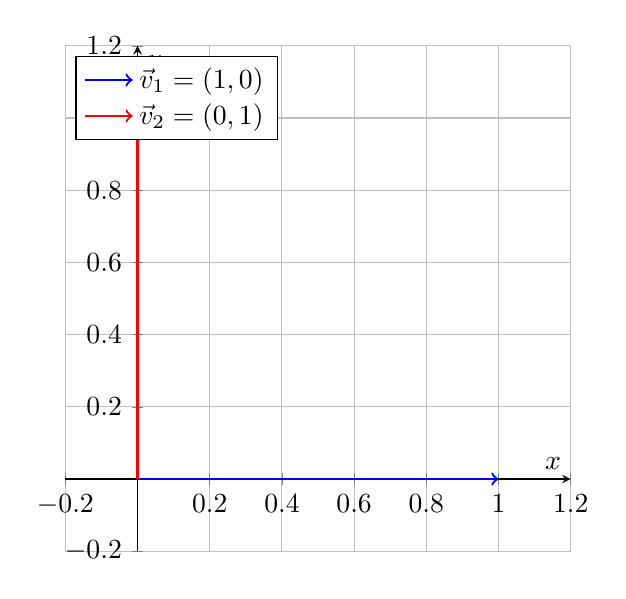
\begin{tikzpicture}
\begin{axis}[
    axis lines = middle,
    xlabel = {$x$},
    ylabel = {$y$},
    xmin = -0.2, xmax = 1.2,
    ymin = -0.2, ymax = 1.2,
    grid = both,
    width=8cm,
    height=8cm,
    legend style={at={(0.02,0.98)},anchor=north west}
]

% Vettore v1 = (1,0)
\addplot[
    ->,
    thick,
    blue
] coordinates {(0,0) (1,0)};
\addlegendentry{$\vec v_1 = (1,0)$}

% Vettore v2 = (0,1)
\addplot[
    ->,
    thick,
    red
] coordinates {(0,0) (0,1)};
\addlegendentry{$\vec v_2 = (0,1)$}

\end{axis}
\end{tikzpicture}
\end{center}

\section{Dimensioni}
Si dice che $V$ (spazio vettoriale) abbia \textbf{dimensione} $n$ se ammette una base di cardinalità $n$. Ogni base di V ha dimensione $n$.
\paragraph{Esempio:}
\[
dim(\mathbb{R}^n) = n
\]
\[
dim(\mathbb{R}^2) = 2
\]
\[
dim(\mathbb{R}[x] \leq d) = d + 1
\]
Supponiamo che $V$ ammetta una base con $n$ elementi e abbiamo $v_1,\ldots,v_r \in V$ con $r > n$ allora $v_1,\ldots,v_r$ sono linearmente dipendenti (uno o più vettori sono superflui) e non possono quindi formare una base.\\
Ogni base di uno spazio vettoriale ha la stessa cardinalità, quindi se abbiamo due basi di $V$:
\[
v_1,\ldots,v_n
\]
\[
e_1,\ldots,e_r
\]
Allora significa che $n = r$.
\paragraph{Dimostrazione:} prendiamo $V = \mathbb{R}^n$, dimostriamo che se $r > n$ allora $v_1,\ldots,v_r \in V$ sono linearmente dipendenti.
\[
v_1 = \begin{bmatrix}
  a_{11}\\
  a_{21}\\
  \ldots\\
  a_{n1}
\end{bmatrix}, v_2 = \begin{bmatrix}
  a_{12}\\
  a_{22}\\
  \ldots\\
  a_{n2}
\end{bmatrix}, \ldots, v_3 = \begin{bmatrix}
  a_{1m}\\
  a_{2m}\\
  \ldots\\
  a_{nm}
\end{bmatrix}
\]
Ricordiamo che se dei vettori sono linearmente dipendenti significa che il sistema omogeneo associato alla matrice costruita con tali vettori ammette almeno una soluzione non banale, ovvero c'è almeno una colonna senza pivot (variabile libera).\\
Notiamo che una volta trovata la forma a scalini con l'algoritmo di Gauss ci saranno $n$ righe e $r$ colonne, ciò vuol dire che ci sono più colonne che righe e quindi almeno una colonna sarà senza pivot, dimostrando che i vettori sono linearmente dipendenti.\\\\
Vediamo adesso il caso contrario, ovvero il caso in cui $r < n$.\\
Sia la dimensione di $V = n$ e siano $w_1,\ldots,w_r \in V$ allora tali vettori sono linearmente indipendenti e il loro span:
\[
Span(w_1,\ldots,w_r) \ne V
\]
Sia la dimensione di $V = n$ e siano $w_1,\ldots,w_r$ linearmente indipendenti, allora:
\[
\exists w_{r+1},\ldots,w_n \in V : w_1,\ldots,w_r,w_{r+1},\ldots,w_n \text{ è una base}
\]
\paragraph{Dimostrazione:} si nota che $Span(w_1,\ldots,w_r) \ne V$, si può trovare quindi un vettore $r+1$ che $\notin Span(w_1,\ldots,w_r)$, dico quindi che $w_1,\ldots,w_r,w_{r+1}$ sono linearmente indipendenti. (appunto se $w_{r+1}$ rendesse la sequenza di vettori linearmente dipendente sarebbe invece incluso nello span)\\
Il fatto che siano linearmente indipendenti è necessario perchè altrimenti l'area coperta dallo span non aumenterebbe e non raggiungerebbe $V$.\\
Per ricondursi alla base, bisogna continuare ad aggiungere vettori fino a che non abbiamo $n$ vettori.\\
Di solito per trovare un nuovo vettore da aggiungere si può controllare la base standard, in quanto è garantito trovare almeno un vettore non è contenuto nello span di $w_1,\ldots,w_r$, infatti se fossero tutti compresi nello span allora anche il loro span lo sarebbe:
\[
Span(base) \subset span(w_1,\ldots,w_r)
\] 
Ma questo è impossibile perchè sappiamo che lo span della base corrisponde a $V$, mentre $Span(w_1,\ldots,w_r) \ne V$, e quindi almeno un vettore della base standard $\notin span(w_1,\ldots,w_r)$\\\\
Se abbiamo $V$ come spazio vettoriale con dimensione $n$ allora $n$ vettori ($r = n$) linearmente indipendenti sono sicuramente base di $V$, in questo caso basta appunto dimostrare l'indipendenza lineare.
\paragraph{Dimostrazione:} siano $v_1,\ldots,v_n \in V$ linearmente indipendenti, devo verificare che $Span(v_1,\ldots,v_n) = V$.\\
Supponiamo per assurdo che $Span(v_1,\ldots,v_n) \ne V$ e quindi:
\[
\exists v_{n+1} \in V : v_{n+1} \notin Span(v_1,\ldots,v_n).
\]
Dimostro allora che $v_1,\ldots,v_n,v_{n+1}$ sono linearmente indipendenti, però è impossibile perchè se i vettori sono più della dimensione dello spazio allora sono linearmente dipendenti, cìo vuol dire che:
\[
\lambda_1 \cdot v_1 + \cdots + \lambda_n \cdot v_n + \lambda_{n+1} \cdot v_{n+1} = 0
\]
Vale solo se $\forall i \lambda_i = 0$, però ci possono essere più casi:
\begin{itemize}
  \item $\lambda_{n+1} \ne 0$ significa che è combinazione lineare degli altri e di conseguenza sarebbe compreso in $Span(v_1,\ldots,v_n)$, cosa impossibile perchè abbiamo supposto il contrario prima.
  \item $\lambda_{n+1} = 0$ significa che $\lambda_1 \cdot v_1 + \cdots + \lambda_n \cdot v_n = 0$, ma siccome $v_1,\ldots,v_n$ sono linearente indipendenti e quindi vale solo se $\forall i \lambda_i = 0$
\end{itemize}
Sia $v_1,\ldots,v_n$ una base di $V$ spazio vettoriale, allora ogni $v \in V$ (vettore / punto nello spazio vettoriale) si scrive in modo unico come:
\[
v = \lambda_1 \cdot v_1 + \cdots + \lambda_n \cdot v_n
\]
\paragraph{Dimostrazione:} siccome $Span(v_1,\ldots,v_n) = V$, $\exists \lambda_1,\ldots,\lambda_n$.\\
Supponiamo che $v^| = \lambda_{1^|} \cdot v_1 + \cdots + \lambda_{n^|} - \cdot v_n$, per sostituzione:
\[
\lambda_1 \cdot v_1 + \cdots + \lambda_n \cdot v_n = \lambda_{1^|} \cdot v_1 + \cdots + \lambda_{n^|} \cdot v_n
\]
\[
(\lambda_ 1 - \lambda_{1^|}) \cdot v_1 + \cdots + (\lambda_n - \lambda_{n^|}) \cdot v_n = 0
\]
Sia $V$ uno spazio vettoriale e $W$ un suo sottospazio:
\[
dim(W) \leq dim(V)
dim(W) = dim(V) \Leftrightarrow W = V
\]
\paragraph{Dimostrazione del punto 1:} abbiamo $w_1,\ldots,w_r \in W$, $dim(V) = n$.
\begin{itemize}
  \item $r > n \implies$ $w_1,\ldots,w_r$ sono linearmente dipendenti in $V$ e quindi anche in $W$, quindi $dim(W) \leq n$. 
\end{itemize}
\paragraph{Dimostrazione del punto 2:} per dimostrare una doppia implicazione dobbiamo dimostrare entrambi i casi:
\begin{itemize}
  \item $V = W \implies dim(W) = dim(V)$, molto semplicemente.
  \item $dim(V) = dim(W) \implies $ se $w_1,\ldots,w_r$ è una base di $W$ allora è un sistema di $n$ vettori linearmente indipendenti in $V$ e quindi anche una base di $V$, quindi $V = W$
\end{itemize}
Questo enunciato vale anche sotto questa forma:
\[
dim(W) < dim(V) \Leftrightarrow W \subsetneq V
\]
\paragraph{Esempio 1:} $V = M_{2X2}$, $W \subset V$ e:
\[
W = \{\begin{bmatrix}
  a_{11} & a_{12}\\
  a_{21} & a_{22}
\end{bmatrix} : a_{12} = a_{21}\}
\]
Ovvero le matrici simmetriche.\\
$Dim(W) = ?$, ovviamente $W \ne V$ perche $V$ contiene sicuramente matrici non simmetriche, quindi $dim(W) < dim(V) \implies dim(W) < 4$.\\
Se guardiamo la base standard delle matrici $2X2$, si trovano due vettori compatibili e linearmente dipendenti per $W$, quindi $2 \leq dim(W) \leq 3$.\\
Possibilmente si può trovare un ulteriore vettore e quindi $Dim(W) = 3$.
\paragraph{Esempio 2:} $V = \mathbb{R}[x]_{\leq 3}$, $dim(V)$ come sappiamo è $=4$ perchè la base standard è $1 + x + x^2 + x^3$, se:
\[
W = \{f \in V : f(1) = 0\}
\]
Allora $W \subset V$, ma anche $W \ne V$ perche $V$ ammette sicuramente polinomi in cui $f(1) \ne 0$, quindi $dim(W) < 4$.\\
Si riescono a trovare tre vettori linearmente dipendenti che soddisfano la proprietà e funzionano come base:
\[
v_1 = x-1
\]
\[
v_2 = (x-1)^2
\]
\[
v_3 = (x-1)^3
\]
Per questo, $dim(W) = 3$
\subsection{Formula di Grassmann}
Stabiliamo prima questo:\\
Se:
\[
v_1 = Span(v_1,\ldots,v_n)
\]
\[
v_2 = Span(w_1,\ldots,w_m)
\]
Allora:
\[
v_1 + v_2 = Span(v_1,\ldots,v_n,w_1,\ldots,w_n)
\]
La \textbf{formula di Grassmann} aiuta a trovare le dimensioni di alcuni spazi vettoriali ed è definita cosi:
\[
Dim(v_1 + v_2) + Dim(v_1 \cap v_2) = Dim(v_1) + Dim(v_2)
\]
\paragraph{Dimostrazione:} graficamente, la somma delle dimensioni di due insiemi ($v_1,v_2$) conta due volte l'intersezione dei due insiemi (se esiste).\\
Per questo $Dim(v_1,v_2)$ da solo manca una quantità dell'intersezione per raggiungere l'eguaglianza.\\
Sia $e_1,\ldots,e_n$ una base di $v_1 \cap v_2$\\
\paragraph{Esempio d'esercizio:}
\[
V = \mathbb{R}^4
\]
\[
v_1 = \begin{cases}
  x_1 + 2x_2 + x_3 = 0\\
  -x_1 - x_2 + 3x_4 = 0
\end{cases}
\]
\[
v_2 = Span(\begin{bmatrix}
  2\\
  0\\
  1\\
  1
\end{bmatrix}, \begin{bmatrix}
  3\\
  -2\\
  -2\\
  0
\end{bmatrix})
\]
\[
Dim(v_1 + v_2) = ?
\]
\[
Dim(v_1 \cap v_2) = ?
\]
Inanzitutto bisogna calcolare le dimensioni di $v_1$ e $v_2$, per $v_2$ è semplice perchè quei vettori sono gia linearmente indipendenti e quindi la dimensione di $v_2$ è 2.\\
La dimensione di $v_1$ va trovata tramite l'algoritmo di Gauss sul sistema omogeneo associato, bisogna contare quante colonne hanno pivot (quanti vettori sono linearmente indipendenti tra loro e formano quindi la base), oppure si possono riscrivere le soluzioni come somma di vettori e contare quanti vettori ci sono.\\
Se diventa troppo difficile si può integrare Gauss-Jordan.\\
Svolgendolo, in questo caso $Dim(v_1) = 2$\\
Adesso si trova la dimensione di $Dim(v_1 + v_2)$ oppure $Dim(v_1 \cap v_2)$, si possono svolgere entrambi ma conviene fare quella che pensiamo sia più semplice.\\
Per trovare la dimensione di $v_1 + v_2$ basta svolgere di nuovo l'algoritmo di Gauss dei vettori di $v_1$ e $v_2$, in questo caso si trova $Dim(v_1 + v_2) = 3$.\\
A questo punto si risolve l'equazione e si trova che $Dim(v_1 \cap v_2) = 1$\\
Se invece si voleva risolvere prima $Dim(v_1 \cap v_2)$, tale insieme corrisponde ai vettori di $v_2$ che soddisfano il sistema di $v_1$, basta sommare i vettori di $v_2$ e sostituire i valori di tale vettore risultante alle variabili del sistema e poi risolverlo normalmente.\\\\
In un caso generale in cui $V_1$ e $V_2$ corrispondono semplicemente a uno span di vettori, per trovare la $Dim(V_1 \cap V_2)$ basta svolgere l'algoritmo di Gauss sul sistema omogeneo associato alla matrice dei vettori di $V_1$ e $-V_2$, trovati i valori di $\lambda$ e $\mu$ (dopo una sostituzione nelle formule delle combinazioni lineari) si trovano i vettori e quindi la dimensione.
\section{Coordinate}
$(\lambda_1,\lambda_2,\ldots,\lambda_n)$ sono le \textbf{coordinate} di $v \in V$ rispetto alla base ordinata $v_1,\ldots,v_n$ (quindi l'ordine dei vettori conta).\\
In parole povere le coordinate di $v$ sono i valori di $\lambda$ per cui la combinazione lineare dei vettori ritorna $v$, ovvero un punto nello spazio o un vettore.\\
\paragraph{Esempio:} coordinate di: 
\[v = \begin{bmatrix}
  0\\
  2\\
  1
\end{bmatrix}\]
in $\mathbb{R}^3$ con la base:
\[
v_1 = \begin{bmatrix}
  1\\
  2\\
  3
\end{bmatrix}, v_2 = \begin{bmatrix}
  1\\
  0\\
  1
\end{bmatrix}, \ldots, v_3 = \begin{bmatrix}
  0\\
  0\\
  1
\end{bmatrix}
\]
Per controllare che sia una base, se non si è sicuri, basta controllare che i vettori siano linearmente indipendenti, in quanto sono 3 vettori e lo spazio è di 3 dimensioni.\\
Per farlo basterebbe svolgere l'algoritmo di Gauss, ma in questo caso evitiamo perchè sappiamo già da un esercizio precedente che è una base.\\
A questo punto si forma la matrice $v_1,v_2,v_3,v$:
\[
\begin{bmatrix}
  1 & 1 & 0 & | & 0\\
  2 & 0 & 0 & | & 2\\
  3 & 1 & 1 & | & 1
\end{bmatrix}
\]
Svolgiamo l'algoritmo di Gauss per sistemi non omogenei:
\[
\begin{bmatrix}
  1 & 1 & 0 & | & 0\\
  0 & -2 & 0 & | & 2\\
  0 & -3 & 1 & | & 1
\end{bmatrix}
\]
\[
\begin{bmatrix}
  1 & 1 & 0 & | & 0\\
  0 & -2 & 0 & | & 2\\
  0 & 0 & 1 & | & -1
\end{bmatrix}
\]
Questa è la matrice in forma a scalini, se risolviamo il sistema associato:
\[
\begin{cases}
  \lambda_1 + \lambda_2 = 0\\
  -2\lambda_2 = 2\\
  \lambda_3 = -1
\end{cases}
\]
\[
\begin{cases}
  \lambda_1 = 1\\
  \lambda_2 = -1\\
  \lambda_3 = -1
\end{cases}
\]
Quindi le coordinate del punto richiesto sono $(1,-1,-1)$

\section{Applicazioni lineari}
Siano $V_1,V_2$ spazi vettoriali, una \textbf{applicazione lineare} di $V_1$ e $V_2$ è una funzione della forma:
\[
\varphi : V_1 \rightarrow V_2
\]
Questa funzione, per essere un'applicazione lineare, deve soddisfare queste due condizioni:
\begin{itemize}
  \item $\varphi(v+w) = \varphi(v) + \varphi(w)$, $\forall v,w \in V_1$
  \item $\varphi(\lambda v) = \lambda \cdot \varphi(v)$, $\forall v \in V_1, \forall \lambda \in \mathbb{R}$
\end{itemize}
Sia $\varphi : V_1 \rightarrow V_2$ un'applicazione lineare, il suo \textbf{nucleo} equivale a:
\[
Ker(\varphi) = \{v_1 \in V_1 : \varphi(v_1) = 0\}
\]
L'\textbf{immagine} di $\varphi$ invece è:
\[
Im(\varphi) = \{v_2 \in V_2 : \exists v_1 \in V_1 : \varphi(v_1) = v_2\}
\]
Sia il nucleo che l'immagine di un'applicazione lineare $\varphi:V_1 \to V_2$ è sottospazi.\\\\
Un'appliczione lineare è unicamente determinata da $\varphi(v_1), \ldots, \varphi(v_n)$ con $v_1,\ldots,v_n$ base di $V_1$.
Questo significa che esiste un solo e unico $\varphi$ tale che:
\[
\varphi(v_1) = w_1 \in V_2, \varphi(v_2) = w_2 \in V_2, \ldots, \varphi(v_n) = w_n \in V_2 
\] 
\paragraph{Esempio:} $V_1 = V_2 = \mathbb{R}^2$
\[
v_1 = \begin{bmatrix}
  1\\
  0
\end{bmatrix}, v_2 = \begin{bmatrix}
  0\\
  1
\end{bmatrix}, w_1 = \varphi(v_1) = \begin{bmatrix}
  1\\
  2
\end{bmatrix}, w_2 = \varphi(v_2) = \begin{bmatrix}
  2\\
  1
\end{bmatrix}
\]
Esiste solo un'applicazione lineare in grado di verificare questi valori, troviamola:\\
Vettore generale in $V_1 = \begin{bmatrix}
  a_1\\
  a_2
\end{bmatrix} = a_1 \cdot \begin{bmatrix}
  1\\
  0
\end{bmatrix} + a_2 \cdot \begin{bmatrix}
  0\\
  1
\end{bmatrix}$\\
Secondo la proposizione precedente, abbiamo che:
\[
\varphi(\begin{bmatrix}
  a_1\\
  a_2
\end{bmatrix}) = a_1\varphi(\begin{bmatrix}
  1\\
  0
\end{bmatrix}) + a_2\varphi(\begin{bmatrix}
  0\\
  1
\end{bmatrix}) = a_1 \cdot \begin{bmatrix}
  1\\
  2
\end{bmatrix} + a_2 \cdot \begin{bmatrix}
  2\\
  1
\end{bmatrix}
\] 
\[
\begin{bmatrix}
  a_1\\
  2a_1
\end{bmatrix} + \begin{bmatrix}
  2a_2\\
  a_2
\end{bmatrix} = \begin{bmatrix}
  a_1 + 2a_2\\
  2a_1 + a_2
\end{bmatrix}
\]
Possiamo notare che l'applicazione lineare è definita da una tabella di coefficienti, la quale di conseguenza è unica per valori specifici, proprio come l'applicazione lineare.\\\\
Se consideriamo $B = (v_1,\ldots,v_n)$ come base di $V_1$ e $B^| = (v_1^|,\ldots,v_n^|)$ come base di $V_2$, la matrice di $\varphi$  rispetto a $B$ in partenza e $B^|$ in arrivo ha questa forma:
\[
\begin{bmatrix}
  a_{11} & \cdots & a_{1m}\\
  \cdots\\
  a_{n1} & \cdots & a_{nm}
\end{bmatrix}
\]
Ogni colonna di questa matrice indica l'immagine di un vettore della base ($\varphi(v_k)$)
Le coordinate di $v \in V_1$ rispetto a $B$ sono:
\[
v = \begin{bmatrix}
  b_1\\
  \cdots\\
  b_n
\end{bmatrix}
\]
E l'immagine (coordinate di $\varphi(v)$ rispetto a $B^|$) è il suo prodotto con la matrice, che è:
\[
M \cdot v = \begin{bmatrix}
  a_{11}b_1 & \cdots & a_{1m}b_m\\
  \cdots\\
  a_{n1}b_1 & \cdots & a_{nm}b_m
\end{bmatrix}
\]
\paragraph{Matrice d'identità:} matrice composta in questo modo:
\[
\begin{bmatrix}
  1 & 0 & \cdots & 0\\
  0 & 1 & \cdots & 0\\
  \cdots\\
  0 & 0 & \cdots & 1
\end{bmatrix}
\]
Questo tipo di matrice viene usata dall'applicazione lineare $\varphi(v) = v, \forall v \in V_1$.\\
Se $B \ne B^|$ allora la matrice non può essere di identità.
\subsection{Trovare immagine e nucleo con la matrice}
\paragraph{Nucleo =} insieme delle soluzioni del sistema omogeneo associato alla matrice.
\paragraph{Immagine = } $Span(\varphi(v_1),\ldots,\varphi(v_n))$, con $B = (v_1,\ldots,v_n)$
Vediamo adesso le dimensioni del nucleo e dell'immagine:
\begin{itemize}
  \item $Dim(Im(\varphi)) = $ colonne con pivot della matrice in forma a scalini
  \item $Dim(Ker(\varphi)) = $ colonne senza pivot della matrice in forma a scalini
\end{itemize}
Da questo possiamo trarre un teorema:
\[
Dim(Ker(\varphi)) + Dim(Im(\varphi)) = Dim(V_1)
\]
Se non ci sono colonne senza pivot, l'immagine copre tutto $V_1$ e quindi $Ker(\varphi) = \emptyset$.
\subsection{Isomorfismo}
Un'applicazione lineare $\varphi: V_1 \to V_2$ è un \textbf{isomorfismo} se:
\begin{itemize}
  \item $Im(\varphi) = V_2$
  \item $\varphi(v_1) = \varphi(v_1^|) \Leftrightarrow v_1 = v_1^|$ (iniettività).
\end{itemize}
Si indica cosi:
\[
\varphi: V_1 \to V_2
\]
Con un $\sim $ sopra la freccetta.\\
C'è un altra condizione, ovvero questo:
\[
Ker(\varphi) = \{0\}
\]
Ovvero che l'immagine è $0$ solo quando $v_1 = 0$.\\\\
Se $\varphi: V_1 \to V_2$ è un isomorfismo, allora esiste un applicazione lineare inversa:
\[
\varPsi:V_2 \to V_1
\]
Tale che la composizione dei due è l'identità di $V_1$ o $V_2$.\\
Se uno spazio vettoriale di dimensione $n$ con base $v_1,\ldots,v_n$, sappiamo che ogni $v \in V$ può essere scritto unicamente come:
\[
v = \lambda_1 \cdot v_1 + \cdots + \lambda_n \cdot v_n
\]
Questo definisce un isomorfismo tra $v \in V$ e le sue coordinate, dato che appunto se $\varphi$ è un isomorfismo $\forall v_2 \in V_2 \exists^| v_1 : \varphi(v_1) = v_2$.\\
Questo vale sia per $\forall v \in V_1$ e $\forall v \in V_2$, si creano quindi due isomorfismi tra i loro nuclei e immagini.

\subsection{Composizione di applicazioni lineari}
Siano $varphi:V_1 \to V_2$ e $\varPsi:V_2 \to V_3$ applicazioni lineari, la loro \textbf{composizione} $\varPsi o \varphi$ è un'applicazione lineare.\\
La matrice di tale composizione corrisponde proprio al prodotto delle matrici delle due applicazioni lineari che sono state composte.\\

\section{Matrici}

\subsection{Prodotto di due matrici}
Sia $A$ una matrice $rxm$ e $B$ una matrice $mxn$, il loro \textbf{prodotto} è definito cosi:
\[
a_{i1} \cdot b_{1j} + \cdots + a_{im} \cdot b_{mj}
\]
Ovvero si moltiplica ogni riga di $A$ con ogni colonna di $B$.\\
Il prodotto di $A$ con una matrice di identità risulta la matrice di $A$, mentre il prodotto con una matrice \textbf{anti-diagonale} è sempre $A$ ma con le colonne scambiate.\\
In generale:
\[
A \cdot B \ne B \cdot A
\]
\[
A \cdot (B \cdot C) = (A \cdot B) \cdot C
\]
\[
A^{-1} = inverso
\]
Il prodotto di $A$ con se stessa $n$ volte è $A^n$ se è d'identità, altrimenti no.\\

\subsection{Rango di una matrice}
Il \textbf{rango} di una matrice $A$ è uguale alla dimensione dell'immagine dell'applicazione lineare a cui è associata.\\
Il rango corrisponde al numero di \textbf{righe non nulle} o de \textbf{pivot} di una matrice una volta portata in forma a scalini.\\
Di conseguenza, corrisponde anche al numero di colonne linearmente indipendenti della matrice.

\subsection{Teorema delle matrici simili}
\[
A^| = PAP^{-1}
\]
Con:
\[
P = id
\]
E le matrici $A$ che sono basate sulle basi $B,B^|$. Si dicono \textbf{simili} se questo è vero. Questo si può dimostrare con la composizione di applicazioni lineari.

\subsection{Riflessione rispetto all'origine}
\[R_0: 
\begin{bmatrix}
  x\\
  y
\end{bmatrix} \to \begin{bmatrix}
  -x\\
  -y
\end{bmatrix}
\]
Matrice di $R_0$ rispetto alla base standard in partenza e arrivo:
\[
\begin{bmatrix}
  1\\
  0
\end{bmatrix} \to \begin{bmatrix}
  -1\\
  0
\end{bmatrix}
\]
\[
\begin{bmatrix}
  \\
  1
\end{bmatrix} \to \begin{bmatrix}
  0\\
  -1
\end{bmatrix}
\]
\[
\begin{bmatrix}
  -1 & 0\\
  0 & -1
\end{bmatrix}
\]
La matrice di $R_0$ o $R_0$ è:
\[
\begin{bmatrix}
  1 & 0\\
  0 & 1
\end{bmatrix}
\]
Ovvero la matrice identità.

\subsection{Riflessione rispetto all'asse x}
\[R_0: 
\begin{bmatrix}
  x\\
  y
\end{bmatrix} \to \begin{bmatrix}
  x\\
  -y
\end{bmatrix}
\]
Matrice rispetto alla base standard in partenza e in arrivo:
\[
\begin{bmatrix}
  1\\
  0
\end{bmatrix} \to \begin{bmatrix}
  1\\
  0
\end{bmatrix}
\]
\[
\begin{bmatrix}
  0\\
  1
\end{bmatrix} \to \begin{bmatrix}
  0\\
  -1
\end{bmatrix}
\]
\[
\begin{bmatrix}
  -1 & 0\\
  0 & -1 
\end{bmatrix}
\]
La matrice di $R_0$ o $R_0$ è:
\[
\begin{bmatrix}
  1 & 0\\
  0 & 1
\end{bmatrix}
\]
Ovvero la matrice identità.\\
In pratica, quando una composizione risulta la matrice di identità allora le matrici composte sono una l'inversa dell'altra, in questo caso l'inverso della matrice di $R_0$ è se stessa.

\subsection{Proiezione all'asse y}
\[\Pi_y: 
\begin{bmatrix}
  x\\
  y
\end{bmatrix} \to \begin{bmatrix}
  x\\
  0
\end{bmatrix}
\]
Matrice rispetto alla base standard in partenza e in arrivo:
\[
\begin{bmatrix}
  1\\
  0
\end{bmatrix} \to \begin{bmatrix}
  1\\
  0
\end{bmatrix}
\]
\[
\begin{bmatrix}
  0\\
  1
\end{bmatrix} \to \begin{bmatrix}
  0\\
  0
\end{bmatrix}
\]
\[
\begin{bmatrix}
  1 & 0\\
  0 & 0 
\end{bmatrix}
\]

\subsection{Rotazione di angolo alfa intorno all'origine}
(questo non è il simbolo corretto, è simile ma con la stanghetta a forma di s)
\[\rho_{\alpha}:\]
Questo sopra è la notazione.\\
Matrice rispetto alla base standard in partenza e in arrivo:
\[
\begin{bmatrix}
  1\\
  0
\end{bmatrix} \to \begin{bmatrix}
  cos(\alpha)\\
  sin(\alpha)
\end{bmatrix}
\]
\[
\begin{bmatrix}
  0\\
  1
\end{bmatrix} \to \begin{bmatrix}
  -sin(\alpha)\\
  cos(\alpha)
\end{bmatrix}
\]
\[
\begin{bmatrix}
  cos(\alpha) & -sin(\alpha)\\
  sin(\alpha) & cos(\alpha) 
\end{bmatrix}
\]
$\rho_{\alpha}$ è un isomorfismo e la sua applicazione lineare inversa è $\rho_{-\alpha}$.
\[
\rho_{\alpha} o \rho_{\alpha} = id
\]

\subsection{Il determinante}
Se $A \in M_{nxn}(\mathbb{R})$, definiamo il \textbf{determinante} di $A$ come $det(A) \in \mathbb{R}$ che ha le seguenti proprietà:
\begin{itemize}
  \item $det(A) = 0 \Leftrightarrow$ le colonne e le righe rispettivamente sono linearmente dipendenti.
  \item $det(A) \ne 0 \Leftrightarrow$ le colonne e le righe rispettivamente sono linearmente indipendenti.
\end{itemize}
Se una matrice $A$ ha $det(A) \ne 0$, allora ammette una matrice inversa $A^{-1}$.\\
Ecco come calcolare il determinante:
\paragraph{n = 1}
$A = [x]$, $det(A) = x$
\paragraph{n = 2}
\[
A = \begin{bmatrix}
  a & b\\
  c & d
\end{bmatrix}
\]
\[
det(A) = ad - bc
\]
Ovvero l'area del parallelogramma associato con lati $(a,c)$ e $(b,d)$.
\paragraph{n > 2}
Il determinante di una matrice $A = [a_{ij}]$ si calcola riconducendosi al caso precedente.\\
$A_{ij} = $matrice ottenuta cancellando la riga $i$ e la colonna $j$.\\
\textbf{Fatto:} tutti questi valori (per ogni $i$) sono uguali e risultano il $det(A)$:
\[
\sum_{j=1}^{n} (-1)^{i+j} \cdot a_{ij} \cdot det(a_{ij})
\]
Per $i fisso$.
\paragraph{Esempio:}
\[
A = \begin{bmatrix}
  1 & 0 & -1\\
  2 & 1 & 0\\
  1 & 0 & 2
\end{bmatrix}
\]
Sviluppiamo rispetto alla prima riga $i = 1$:
\[
1 \cdot det(\begin{bmatrix}
  1 & 0\\
  0 & 2
\end{bmatrix}) - 0 \cdot det(\begin{bmatrix}
  2 & 0\\
  1 & 2\\
\end{bmatrix}) - 1 \cdot det(\begin{bmatrix}
  2 & 1\\
  1 & 0
\end{bmatrix})
\]
Ognuna di queste sottomatrici sono gli elementi rimasti dall'eliminazione della colonna e riga dove si trovava l'elemento selezionato ($j$).\\\\
Le matrici dove è facile calcolare il determinante sono:
\begin{itemize}
  \item Matrici con almeno una colonna o riga $= 0$.
  \item Se $A$ è una matrice triangolare superiore, ovvero che tutti gli elementi sotto la diagonale sono $= 0$ (ovvero con $i > j$), allora:
  \[
  det(A) = a_{11} \cdot a_{22} \cdot \ldots \cdot a_{nn}
  \]
  Ovvero tutti i numeri sulla diagonale.\\
  Vale lo stesso per le matrici diagonali inferiori.
  \item Se $A$ è una matrice diagonale (di identità), $det(A) = 1$.
\end{itemize}
Se scambio due righe adiacenti, il determinante cambia segno.\\
Lo scambiare due righe non adiacenti corrisponde a fare scambi adiacenti più volte, e quindi cambiare il segno più volte.\\
Se le righe adiacenti scambiate sono uguali, il segno non cambia, questo perchè:
\[
\text{Almeno due righe uguali} \Leftrightarrow det(A) = 0
\]
Il segno in realtà cambia, ma rimane invariato perchè $det(A) = 0$.
\subsection{Matrice aggiunta}
La matrice aggiunta di $A$ è:
\[
\tilde{A} = [\tilde{a}_{ij}]
\]
Dove:
\[
\tilde{a}_{ij} = (-1)^{i+j} \cdot det(A_{ij})
\]
\subsection{Formula di Kramer:}
\[
A \cdot \tilde{A} = det(A) \cdot I = \begin{bmatrix}
  det(A) & 0 & 0\\
  0 & det(A) & 0\\
  0 & 0 & det(A)
\end{bmatrix}
\]
Se $det(A) \ne 0$ allora esiste una matrice inversa:
\[
A^{-1} = \frac{1}{det(A)} \cdot \tilde{A}
\]
\subsection{Dim di Cramer (non ho idea di cosa sia "dim")}
\[
\text{riga i di A} \cdot \text{colonna j di A} = det(A)
\]
Se $i = j$, altrimenti $= 0$.
\subsection{Teorema di Binet o Cauchy}
\[
det(A \cdot B) = det(A) \cdot det(B)
\]
\subsection{Altro teorema}
Per $A \in M_{nxn}(\mathbb{R})$ sono equivalenti (valgono tutte insieme):
\begin{itemize}
  \item $\exists A^{-1}$
  \item $det(A) \ne 0$
  \item colonne e righe di $A$ sono linearmente indipendenti
\end{itemize}
\subsection{Matrice trasposta}
La matrice trasposta di $A = [a_{ij}]$ è:
\[
A^t = [a_{ji}]
\]
Ovvero riga $i$ di $A^t =$ colonna $i$ di $A$.\\
Dato il teorema precedente si può dire:
\[
det(A^t) = det(A)
\]
\subsection{Altra proposizione}
Se $\varphi: V \to V$ è un applicazione lineare, $B,B^|$ basi di $V$ (spazio vettoriale), $A =$ matrice di $\varphi$ rispetto a $B$ in partenza e arrivo e $A^|$ analogo, allora $det(A) = det(A^|)$.
\paragraph{Dimostrazione:}
\[
A^| = PAP^{-1}
\]
\[
det(A^|) = det(PAP^{-1})
\]
\[
det(P) \cdot det(A) \cdot det(P^{-1}) = det(A)
\]
\[
det(A^|) = det(A)
\]
\subsection{Teorema rango-nullità}
Il teorema specifica questo per una matrice $A$:
\[
dim(Ker(A)) = n - rango(A)
\]
Dove $n$ è il numero di variabili distinte dello spazio vettoriale / applicazione lineare associati.

\section{Autovalori e autovettori}
Dato $V$ uno spazio vettoriale con $dim(V) < \infty$ e $\varphi:V \to V$ un'applicazione lineare, $\lambda \in \mathbb{R}$ è \textbf{autovalore} se:
\[
\exists v \in V \ne 0 : V: \varphi(v) = \lambda \cdot v
\]
Tale $v$ si chiama \textbf{autovettore} di $\varphi$ per $\lambda$.\\
\begin{itemize}
  \item Un $v \ne 0$ può essere autovettore di un solo $\lambda$ al massimo, infatti se:
  \[
  \varphi(v) = \lambda_1 \cdot v
  \]
  \[
  \varphi(v) = \lambda_2 \cdot v
  \]
  \[
  \lambda_1 \cdot v = \lambda_2 \cdot v
  \]
  \[
  (\lambda_1 + \lambda_2) \cdot v = 0
  \]
  \[
  v \ne 0 \implies \lambda_1 = \lambda_2
  \]
  \item Per $\lambda$ fisso, esistono molteplici autovettori per $\lambda$.
  \[
  \varphi = id
  \]
  \[
  \forall v
  \]
  \[
  \varphi(v) = 1 \cdot v
  \]
  \item Esiste un numero finito di autovalori ($\leq dim(V)$)
\end{itemize}
Se $\lambda$ è autovalore di $\varphi$, gli autovettori per $\lambda$ e il vettore $0$ formano un sottospazio di $V$ chiamato \textbf{autospazio} di $\lambda$ e si denota $V_{\lambda}$.
\paragraph{Dimostrazione: }come sappiamo un sottospazio deve soddisfare due condizioni, ovvero che la somma di vettori e il prodotto scalare di un vettore fanno parte anchessi del sottospazio oltre i vettori usati.\\
Dimostriamo gli autospazi:\\
\[
v_1,v_2 \in V_{\lambda} \Leftrightarrow \varphi(v_1) = \lambda \cdot v_1, \varphi(v_2) = \lambda \cdot v_2
\]
\[
\varphi(v_1 + v_2) = \varphi(v_1) + \varphi(v_2) = \lambda \cdot v_1 + \lambda v_2 = \lambda(v_1 + v_2) \Leftrightarrow v_1, v_2 \in V_{\lambda}
\]
\[
\varphi(\alpha \cdot v) = \alpha \cdot \varphi(v) = \alpha \cdot \lambda \cdot v = \lambda(\alpha \cdot v) \implies \alpha \cdot v \in V_{\lambda}
\]

\section{Diagonalizzabilità}
$\varphi$ è diagonalizzabile se esiste una base di $V$ dove la matrice di $\varphi$ (in partenza e arrivo) è diagonale.\\
$\varphi$ è diagonalizzabile se e solo se esiste una base di $V$ costituita da autovettori di $\varphi$.
\paragraph{Dimostrazione:} $\varphi$ è diagonalizzabile se e solo se esiste una base $v_1,\ldots,v_n$ dove:\\
\[
A = \begin{bmatrix}
  \lambda_1 & \ldots & 0\\
  \ldots\\
  0 & \ldots & \lambda_n
\end{bmatrix}
\]
Se appunto esiste una base del genere con tale matrice, allora l'applicazione lineare è questa:
\[
\varphi(v_k) = \lambda_k \cdot v_k
\]
Ovvero le coordinate di un vettore sono la colonna $k$ della matrice, questo dimostra che ogni vettore è autovettore e se partiamo invece dall'applicazione lineare, se proviamo a ricostruire la matrice associata ritroviamo proprio questa riportata sopra.
\paragraph{Proposizione:} $A \in M_{nxn}(\mathbb{R})$ è diagonalizzabile $\Leftrightarrow$ esiste $P$ invertibile tale che $PAP^{-1} = D$, con $D = $ matrice diagonale.
\paragraph{Applicazione:} sia $A \in M_{nxn}(\mathbb{R})$, calcola $A^{2026}$.\\
\begin{itemize}
  \item Se $A$ è diagonale, allora:
  \[
  A^{2026} = \begin{bmatrix}
    \lambda_1^{2026} & \ldots & 0\\
    \ldots\\
    0 & \ldots & \lambda_n^{2026}
  \end{bmatrix}
  \]
  \item Se $A$ è diagonalizzabile, allora:
  \[
  PAP^{-1} = D \Leftrightarrow A = P^{-1}DP
  \]
  \[
  A^{2026} = P^{-1}DP \cdot P^{-1}DP \cdot P^{-1}DP \cdot \ldots = P^{-1}D^{2026}P
  \]
\end{itemize}
Quindi questo esempio di applicazione dimostra quanto questi teoremi facilitino tali calcoli enormi.
\subsection{Indipendenza lineare di autovettori}
Supponiamo $\lambda_1,\ldots,\lambda_r$ autovalori distinti di $\varphi$ e $v_i$ autovettore per $\lambda_i$ per ogni $i$ e $\varphi(v_i) = \lambda_i \cdot v_i$ allora $v_1,\ldots,v_r$ sono linearmente indipendenti.\\
Se $\varphi$ ammette $n = dim(V)$ autovalori distinti allora $\varphi$ è diagonalizzabile (non sempre vero il contrario).\\
In breve, autovettori per autovalori distinti sono sempre linearmente indipendenti.
\paragraph{Dimostrazione:}per definizione, i vettori sono linearmente indipendenti se l'unica combinazione lineare che dà il vettore nullo è quella con tutti i coefficienti nulli. \\
Supponiamo quindi che esista una combinazione lineare nulla:
\[
a_1 v_1 + a_2 v_2 + \dots + a_k v_k = 0.
\tag{1}
\]
Dobbiamo dimostrare che
\[
a_1 = a_2 = \dots = a_k = 0.
\]
Applichiamo l'applicazione lineare $\phi$ a entrambi i membri della (1):
\[
\phi(a_1 v_1 + a_2 v_2 + \dots + a_k v_k) = \phi(0).
\]
Poiché $\phi$ è lineare:
\[
a_1 \phi(v_1) + a_2 \phi(v_2) + \dots + a_k \phi(v_k) = 0.
\]
Poiché i vettori sono autovettori:
\[
\phi(v_i) = \lambda_i v_i,
\]
quindi otteniamo:
\[
a_1 \lambda_1 v_1 + a_2 \lambda_2 v_2 + \dots + a_k \lambda_k v_k = 0.
\tag{2}
\]
Ora abbiamo le due equazioni:
\[
\begin{cases}
a_1 v_1 + a_2 v_2 + \dots + a_k v_k = 0 \\
a_1 \lambda_1 v_1 + a_2 \lambda_2 v_2 + \dots + a_k \lambda_k v_k = 0
\end{cases}
\]
Moltiplichiamo la prima equazione per $\lambda_1$:
\[
a_1 \lambda_1 v_1 + a_2 \lambda_1 v_2 + \dots + a_k \lambda_1 v_k = 0.
\tag{3}
\]
Ora sottraiamo la (3) dalla (2):
\[
(2) - (3).
\]
Otteniamo:
\[
(a_1 \lambda_1 v_1 - a_1 \lambda_1 v_1)
+ (a_2 \lambda_2 v_2 - a_2 \lambda_1 v_2)
+ \dots +
(a_k \lambda_k v_k - a_k \lambda_1 v_k)
= 0.
\]
Il primo termine si annulla:
\[
a_1 \lambda_1 v_1 - a_1 \lambda_1 v_1 = 0.
\]
Negli altri termini raccogliamo:
\[
a_2(\lambda_2 - \lambda_1)v_2 + a_3(\lambda_3 - \lambda_1)v_3 + \dots + a_k(\lambda_k - \lambda_1)v_k = 0.
\tag{4}
\]
Poiché gli autovalori sono distinti:
\[
\lambda_i - \lambda_1 \neq 0 \quad \text{per } i \neq 1.
\]
Quindi la (4) è una combinazione lineare dei vettori
$v_2, \dots, v_k$ uguale a zero.\\
Ripetendo lo stesso procedimento, moltiplichiamo la (4) per
$\lambda_2$ e sottraiamo l'equazione ottenuta applicando $\phi$
alla (4), eliminando così $v_2$.\\
Continuando questo procedimento si ottiene infine:
\[
a_k(\lambda_k - \lambda_{k-1}) v_k = 0.
\]
Poiché $v_k \neq 0$ e $\lambda_k \neq \lambda_{k-1}$, segue che
\[
a_k = 0.
\]
Sostituendo a ritroso nelle equazioni precedenti si ottiene:
\[
a_{k-1} = 0, \dots, a_1 = 0.
\]
Quindi:
\[
a_1 = a_2 = \dots = a_k = 0.
\]
Pertanto i vettori $v_1, \dots, v_k$ sono linearmente indipendenti.\hfill $\square$
\subsection{Proposizione delle dimensioni degli autospazi}
Supponiamo che gli autovalori di $\varphi$ sono $\lambda_1,\ldots,\lambda_n$, allora $\varphi$ è diagonalizzabile se e solo se:
\[
dim(V_{\lambda_1}) + dim(V_{\lambda_2}) + \ldots + dim(V_{\lambda_n}) = dim(V)
\]
\paragraph{Dimostrazione:}Sia $\phi : V \to V$ un'applicazione lineare e siano 
$\lambda_1, \dots, \lambda_k$ gli autovalori distinti con i relativi autospazi 
\[
E_{\lambda_i} = \{ v \in V : \phi(v) = \lambda_i v \}.
\]
\textbf{Step 1: intersezione banale degli autospazi.}  
Mostriamo che se $i \neq j$, allora 
\[
E_{\lambda_i} \cap E_{\lambda_j} = \{0\}.
\] 
Sia $v \in E_{\lambda_i} \cap E_{\lambda_j}$. Allora
\[
\phi(v) = \lambda_i v \quad \text{e} \quad \phi(v) = \lambda_j v.
\]
Sottraendo, otteniamo
\[
\lambda_i v - \lambda_j v = (\lambda_i - \lambda_j)v = 0.
\]
Poiché $\lambda_i \neq \lambda_j$, segue $v = 0$.  
Quindi ogni coppia di autospazi con autovalori diversi si interseca solo nello zero.\\
(In pratica, se moltiplichiamo un valore per due valori diversi, i risultati saranno uguali solo se il primo valore è nullo)\\
\textbf{Step 2: linearmente indipendenti.}  
Sia $\{v_{i1}, \dots, v_{in_i}\}$ una base di $E_{\lambda_i}$ per ogni $i$. Consideriamo l’unione di tutte le basi:
\[
\{v_{11},\dots,v_{1n_1},v_{21},\dots,v_{2n_2},\dots,v_{k1},\dots,v_{kn_k}\}.
\] 
Supponiamo che esista una combinazione lineare nulla:
\[
\sum_{i=1}^{k} \sum_{j=1}^{n_i} a_{ij} v_{ij} = 0.
\] 
Raggruppando i termini per autospazi, otteniamo
\[
w_1 + w_2 + \dots + w_k = 0, \quad w_i \in E_{\lambda_i}.
\] 
Poiché l’intersezione tra $E_{\lambda_i}$ e la somma degli altri autospazi è solo $\{0\}$, segue che
\[
w_1 = w_2 = \dots = w_k = 0.
\] 
Pertanto tutti i coefficienti $a_{ij} = 0$ e i vettori sono linearmente indipendenti.\\
\textbf{Step 3: somma delle dimensioni.}  
Abbiamo quindi $n_1 + \dots + n_k$ vettori linearmente indipendenti. Se questi riempiono lo spazio $V$, cioè
\[
n_1 + \dots + n_k = \dim V,
\] 
allora la somma degli autospazi è diretta e forma una base di $V$. In altre parole,
\[
V = E_{\lambda_1} \oplus \dots \oplus E_{\lambda_k},
\]
e la dimensione totale della somma degli autospazi è
\[
\dim E_{\lambda_1} + \dots + \dim E_{\lambda_k} = \dim V.
\]
\textbf{Conclusione.}  
Questo mostra che un applicazione lineare è diagonalizzabile se e solo se la somma delle dimensioni degli autospazi è uguale alla dimensione dello spazio vettoriale, grazie all’indipendenza degli autovettori e all’intersezione banale degli autospazi relativi ad autovalori distinti.
\subsection{Come trovare gli autovalori}
Per capire se un applicazione lineare è diagonalizzabile, bisogna trovare gli autovalori e poi una base per ciascun autospazio.\\
Per trovare gli autovalori teniamo a mente che:
\[
\lambda \text{ è autovalore} \Leftrightarrow \exists v \ne 0 : \varphi(v) = \lambda \cdot v
\]
Parte di questo si riscrive come:
\[
\varphi(v) - \lambda \cdot v
\]
Consideriamo l'applicazione lineare $\varphi - \lambda \cdot id$, la sua matrice sarà:
\[
A = \begin{bmatrix}
  a_{11} - \lambda & \ldots & a_{1n}\\
  \ldots\\
  a_{n1} & \ldots & a_{nn} - \lambda
\end{bmatrix}
\]
Ovvero viene sottratto $\lambda$ ai valori sulla diagonale identità.\\
Adesso diciamo che $v$ è autovettore di $\varphi$ per $\lambda$ se e solo se:
\begin{itemize}
  \item $Ker(\varphi - \lambda \cdot id) \ne 0$ (contiene $v = 0$)
  \item $det(\varphi - \lambda \cdot id) = det(A - \lambda \cdot I) = 0$ ($I$ è matrice identità) 
\end{itemize}
\paragraph{Esempio:}
\[ A = 
\begin{bmatrix}
  1 & 1\\
  0 & 1
\end{bmatrix}
\]
\[
A - \lambda = \begin{bmatrix}
  1 - \lambda & 1\\
  0 & 1 - \lambda
\end{bmatrix}
\]
Il determinante è $(1-\lambda)^2$, deve essere nullo per fare in modo che $\lambda$ sia autovalore, in questo caso l'unico autovalore è $0$.
\subsection{Polinomio caratteristico}
Il \textbf{polinomio caratteristico} di $A$ è:
\[
det(A - \lambda \cdot I) \in \mathbb{R}[t]
\]
Gli autovalori sono le radici del polinomio caratteristico, ovvero i valori per cui il polinomio è nullo.\\
Se $A$ è la matrice di $\varphi:V \to V$ applicazione lineare rispetto ad una base allora il polinomio caratteristico non dipende dalla base se e solo se da un altra base si ottiene lo stesso polinomio.
\paragraph{Dimostrazione:} Se $B$ è la matrice di $\varphi$ rispetto ad'un altra base, sappiamo che:
\[
B = PAP^{-1}
\]
Per un certo $P$.
\[
det(B - \lambda \cdot I) = det(PAP^{-1} - \lambda \cdot I) = det(PAP^{-1} - \lambda \cdot P \cdot P^{-1}) = \ldots
\]
\[
\ldots = det(P(A - \lambda(A - \lambda \cdot I)P^{-1})) = det(P) \cdot det(A-\lambda \cdot I) \cdot det(P^{-1})
\]
\subsection{Come trovare gli autovettori}
Una volta trovati i nostri autovalori, per trovare gli autovettori per ogni autovalore bisogna:
\begin{enumerate}
  \item Scegliere un autovalore ($\lambda  = k$)
  \item Impostare questa equazione:
  \[
  (A - \lambda \cdot I) \cdot \begin{bmatrix}
    x_1\\
    x_2\\
    \ldots\\
    x_n
  \end{bmatrix} = \lambda \cdot \begin{bmatrix}
    x_1\\
    x_2\\
    \ldots\\
    x_n
  \end{bmatrix} 
  \]
  \item Svolgere il sistema associato
\end{enumerate}
Una volta trovate le soluzioni, bisogna guardare la base standard delle soluzioni, quelli sono gli autovettori.\\
Ricordiamo che le dimensioni di tutti gli autospazi deve risultare la dimensione dello spazio vettoriale $V$.\\
Per trovare le dimensioni degli autospazi bisogna proprio effettuare il teorema del rango-nullità:
\[
dim(V_{\lambda}) = dim(Ker(A_{\lambda})) = nVar - rango(A_{\lambda})
\]
Dove $A_{\lambda}$ è la matrice associata al sistema risultante del passaggio sopra.\\\\
Una volta trovati gli autovettori, se la somma delle dimensioni di tutti gli autospazi corrisponde alla dimensione totale e quindi $A$ / $\varphi$ è diagonalizzabile allora possiamo stabilire una matrice simile secondo la base generata dagli autovettori trovati:
\[
A^| = \begin{bmatrix}
  \lambda_1 & \ldots & 0\\
  \ldots\\
  0 & \ldots & \lambda_n
\end{bmatrix}
\]
Dove $\lambda_i$ è autovalore.
\subsection{Esempi di esercizi}
\paragraph{Esempio 1}
\[
A = \begin{bmatrix}
  1 & 1 & 0\\
  0 & 0 & 1\\
  0 & 0 & -1
\end{bmatrix}
\]
\[
\varphi:\mathbb{R}^3 \to \mathbb{R}^3
\]
Troviamo gli autovalori, essi corrispondono alle \textbf{radici} del polinomio caratteristico.\\
\[
det(A - \lambda \cdot I) = \begin{bmatrix}
  1-\lambda & 1 & 0\\
  0 & -\lambda & 1\\
  0 & 0 & -1 - \lambda
\end{bmatrix}
\]
Questa è una matrice triangolare superiore, quindi il determinante è uguale al prodotto di tutti gli elementi sulla diagonale:
\[
(1-\lambda)(-\lambda)(-1-\lambda)
\]
I valori che annullano questo polinomio (e quindi gli autovalori), sono:
\[
\lambda = \{1,0,-1\}
\]
Per determinare se $A$ è diagonalizzabile, bisogna controllare se, come dice il teorema, tutti gli autovettori per tutti gli autovalori sono tanti quanti la dimensione dello spazio vettoriale.\\
Quindi, la somma delle dimensioni degli autospazi deve risultare la dimensione di $\mathbb{R}^3$ in questo caso, ovvero $3$.
\paragraph{Autospazio per 1}
\[
\begin{bmatrix}
  1 & 1 & 0\\
  0 & 0 & 1\\
  0 & 0 & -1
\end{bmatrix} \cdot \begin{bmatrix}
  x\\
  y\\
  z
\end{bmatrix} = 1 \cdot \begin{bmatrix}
  x\\
  y\\
  z
\end{bmatrix}
\]
\[
\begin{cases}
  x + y = x\\
  z = y\\
  -z = z
\end{cases}
\]
\[
\begin{cases}
  x = \text{ qualsiasi}\\
  y = 0\\
  z = 0
\end{cases}
\]
Questo è nella forma:
\[
\begin{bmatrix}
  x\\
  0\\
  0
\end{bmatrix} \text{ multiplo di: } \begin{bmatrix}
  1\\
  0\\
  0
\end{bmatrix}
\]
Quest'ultimo è un autovettore, l'unico per $\lambda = 1$.\\
La dimensione dell'autospazio $V_{\lambda_1}$ è quindi $1$.\\
Se svolgiamo anche gli altri autovalori, troviamo altri 2 autovettori, per un totale di 3, questo ci conferma che la matrice è diagonalizzabile.
Se invece gli autovettori fossero stati di meno, allora no.
\subsection{Molteplicità}
Prima di spiegare la molteplicità introduciamo una proposizione.\\
Se $f \ne 0$, $a$ è radice di $f$ se:
\[
f = (t - a) \cdot g
\] 
\[
deg(g) = deg(f) - 1
\]
\paragraph{Esempio:}
\[
f = t^2 + t
\]
\[
f(0) = 0
\]
\[
f = (t - 0)(t + 1)
\]
Quindi possiamo dire:
\[
f(a) = 0 \implies \exists m > 0 : f = (t - a)^m \cdot g
\]
Con $g(a) \ne 0$ (a non è radice in g).
\paragraph{Dimostrazione:}
\[
f = (t - a) \cdot g_1
\]
\begin{itemize}
  \item Se $g_1(a) \ne 0$ allora tutto è dimostrato.
  \item $g_1(a) = 0$ allora il teorema si riapplica a $g_1$ fino a che non si verifica il punto precedente. Ricordiamo che il grado di $g$ diminuisce sempre di 1 e quindi non ce ne sono infiniti.
\end{itemize}
Questo $m$ quan sopra è la \textbf{molteplicita} della radice $a$ di $f$.\\
Supponiamo che $a_1$ è radice di $f = (t - a_1)^m \cdot g$ di molteplicita $m$ e $a_2$ un'altra radice di $f$, allora:
\[
g(a_2) = 0
\]
Perchè:
\[
0 = f(a_2) = (a_2 - a_1)^m \cdot g(a_2)
\]
E perche in tale equazione $a_2 - a_1$.\\
\subsubsection{Molteplicità algebrica e geometrica}
Sia $\varphi: V \to V$ un'applicazione lineare e $\lambda$ come autovalore di $\varphi$, la \textbf{molteplicita algebrica} di $\lambda$ è la sua molteplicita come radice del polinomio caratteristico.\\
La \textbf{molteplicita geometrica} di $\lambda$ è $dim(V_{\lambda})$.\\
Per queste definizioni vale questo:
\[
moltAlg(\lambda) \geq moltGeom(\lambda)
\]
Questo è interessante perche se la molteplicita algebrica di un autovalore è $1$, allora anche la molteplicita geometrica sarà $1$.\\
Inoltre, la somma di tutte le molteplicita algebriche di tutti gli autovalori è uguale a $n = dim(V)$.
\subsection{Numeri complessi}
Un \textbf{numero complesso} è un espressione $z = a + bi$ dove $a,b \in \mathbb{R}$, $i$ parametro della formula per cui:
\[
i^2 = -1
\]
Questi numeri servono per risolvere alcuni problemi.\\
Per esempio, una matrice potrebbe non essere diagonalizzabile in $\mathbb{R}$, ma potrebbe esserlo in $\mathbb{C}$ (insieme dei numeri complessi).\\
Per definizione, l'insieme $\mathbb{R}$ è sottoinsieme di $\mathbb{C}$.\\
L'insieme $\mathbb{C}$ ammette queste operazioni:\\
Se:
\[
z = a + bi
\]
\[
z^| = a^| + b^|i
\]
Allora valgono queste operazioni:
\begin{itemize}
  \item Somma
  \[
  (z + z^|) = (a + a^|) + (b + b^|)i
  \]
  \item Prodotto per $\lambda \in \mathbb{R}$
  \[
  \lambda z = \lambda a + \lambda bi
  \]
\end{itemize}
Da questo si deduce che $\mathbb{C}$ è uno spazio vettoriale e ha quindi una base di dimensione $2$:
\[
1 + i
\]
Inoltre si può svolgere il prodotto tra numeri complessi:
\[
z \cdot z^| = (a + bi)(a^| + b^|i) = (a \cdot a^| - b \cdot b^|)(ab^| + a^|b)i
\]
\paragraph{Esempio:}
\[
i^2 = (0 + i)(0 + i) = -1 + 0 \cdot i = -1
\]
\subsubsection{Coniugati}
Se $z = a + bi$, il suo coniugato è:
\[
\overline{z} = a - bi
\]
Si osserva:
\[
z + \overline{z} = 2a \in \mathbb{R}
\]
\[
z \cdot \overline{z} = a^2 + b^2 \in \mathbb{R}
\]
Se $z \ne 0$ allora:
\[
\frac{1}{z} = \frac{\overline{z}}{a^2 + b^2}
\]
E anche:
\[
\frac{z^|}{z} = \frac{z^| \cdot \overline{z}}{a^2 + b^2}
\]
Se $\Delta \in \mathbb{R}$, $\Delta < 0 \implies -\Delta > 0$ allora:
\[
\exists \sqrt{-\Delta}
\]
\[
\sqrt{\Delta \cdot i}^2 = -\Delta \cdot (-1) = \Delta
\]
Possiamo dire che a questo punto ogni polinomio in $\mathbb{C}$ ammette radici.\\
\subsection{Teorema fondamentale dell'algebra}
Il teorema dice questo:
\[
f \in \mathbb{C}[t] \implies \exists z \in \mathbb{C} : f(z) = 0
\]
Questo significa che ogni polinomio in $\mathbb{C}[t]$ (e quindi anche in $\mathbb{R}[t]$) ha almeno una radice complessa.\\
Se questo si avvera ed esiste una radice $z$ per cui $f(z) = 0$, allora anche $f(\overline{z}) = 0$.\\
Il teorema di conseguenza indica che una funzione qualsiasi ha sempre almeno un autovalore in $\mathbb{C}$.
\end{document}